\documentclass[12pt]{article}
\usepackage[utf8]{inputenc}
\usepackage{amsmath}
\usepackage{algpseudocode}
\usepackage{algorithm}
\usepackage{listings}
\usepackage{geometry}
\usepackage{graphicx}
\usepackage{appendix}
\usepackage{subfig}
\usepackage{subcaption}
\usepackage{gensymb}
\usepackage{cancel}
\usepackage{physics}
\usepackage[square, numbers]{natbib}
\usepackage[colorlinks=true]{hyperref}
\usepackage{xcolor}
\makeatletter
\def\l@section{\@dottedtocline{1}{1em}{2em}}
\makeatother
\makeatletter
\def\l@subsection{\@dottedtocline{1}{1em}{3em}}
\makeatother
\hypersetup{
  colorlinks,
  citecolor=.}
\definecolor{codegreen}{rgb}{0,0.6,0}
\definecolor{codegray}{rgb}{0.5,0.5,0.5}
\definecolor{codepurple}{rgb}{0.58,0,0.82}
\definecolor{backcolour}{rgb}{0.95,0.95,0.92}
\lstdefinestyle{mystyle}{
    backgroundcolor=\color{backcolour},   
    commentstyle=\color{codegreen},
    keywordstyle=\color{magenta},
    numberstyle=\tiny\color{codegray},
    stringstyle=\color{codepurple},
    basicstyle=\ttfamily\footnotesize,
    breakatwhitespace=false,         
    breaklines=true,                 
    captionpos=b,                    
    keepspaces=true,                 
    numbers=left,                    
    numbersep=5pt,                  
    showspaces=false,                
    showstringspaces=false,
    showtabs=false,                  
    tabsize=2
}

\lstset{style=mystyle}


\begin{document}
\pagenumbering{gobble}
\thispagestyle{empty}
\begin{center} \vspace{1cm}
    \textbf{\Large{Studies of Hamiltonians using \\
various Neural Network architectures}}\\ \vspace{0.5cm}
    \small{by}\\ \vspace{0.5cm}
    \large{Simen Løken}\\ \vspace{4.4cm}
    \large{THESIS}\\ \vspace{0.3cm}
    \small{for the degree of}\\ \vspace{0.3cm}
    \large{MASTER OF SCIENCE}\\ \vspace{0.7cm}
    \includegraphics[scale=1.0]{DUO_UiO_segl.png} \\ \vspace{0.5cm}
    \large{Faculty of Mathematics and Natural Sciences \\ University of Oslo} \\ \vspace{0.5cm}
    \small{June 2024}\\ \vfill
\end{center}
\newpage
\vspace*{\fill}
{\setlength{\parindent}{0cm}
\renewcommand \thepart{\arabic{part}}
\renewcommand \thesection{\arabic{part}.\arabic{section}}
\definecolor{direct-cite}{gray}{0.1}

\counterwithin*{section}{part}
\numberwithin{equation}{part}
%\numberwithin{equation}{section}
\numberwithin{figure}{part}


\nocite{qmbook1}
\nocite{qmbook2}
\nocite{fys2140}
\nocite{fys3110}
\nocite{fys3150}
\nocite{fys4411}
\nocite{fysstk3155}
\nocite{fys5429}
\nocite{gab}
\nocite{zaheer2018deepsets}

\newpage
\part*{Abstract}
In this work, we from build from the ground a series of software with which we may study various Hamiltonians using a Variational Monte Carlo approach. We do this by first building a theoretical understanding of what the Variational Monte Carlo is, how it works and where it comes from, before then building layer by layer until we arrive at a complete understanding of the Variational Monte Carlo method and how to employ it. \newline
We then employ the theory for two distinct neural network architectures: A Restricted Boltzmann Machine using JAX and a Feed-Forward Neural Network using PyTorch. We find that many of the systems can be accurately modelled using these networks, which in turn is very promising as one of the most difficult problems of traditional Variational Monte Carlo is the selection of a sufficiently good wave function ansatz, which this method bypasses entirely by automating the process.
\newline
We hope therefore that this approach enhances the accessilibity and applicability of Variational Monte Carlo, but also underscores the potential of employing neural networks to streamline and optimize computational methods in quantum mechanics.
\newpage
\part*{Acknowledgements}
As I near the end of my studies, I would like to extend thanks and acknowledgements to everyone who as been helpful throughout my studies. Firstly I would like to extend a massive thank you to my supervisor, Morten Hjorth-Jensen, for being incredibly helpful and knowledgeable about any issues I may have. If it hadn't been for your FYS3150 and FYS-STK3155 courses, both of which I took in the autumn of 2020, I would've never dreamed of pursuing a Master's Degree.
\newline
I would like to extend a thanks to my friends whom I've always been able to lean on when I've needed a break from my studies. Special thanks to player\textunderscore cs\textunderscore gutta whom I've had many \textit{interesting}, \textit{lively} and not to mention \textit{funny} conversations with, be it day or night. \newline
I would also like to extend a thanks to my immediate family, my mom, my dad and my sister, who've been helpful emotional and motivational support over these last years. \newline Lastly I would like to extend a thanks to my grandparents, who are always welcoming if I ever need a break from studying, or if I just want something good to eat.
\newpage
~\newpage
{
  \hypersetup{linkcolor=black}
  \tableofcontents
}

\newpage
~\newpage
\part{Introduction}
\pagenumbering{arabic}

\section{Quantum Mechanics}
When talking about the origins of Quantum Mechanics, it is often viewed through the lens of a dramatic rift between the pre-existing classical physics, and that of the new quantum theory. Indeed, many of the central pillars of quantum mechanics, such as its discreteness and indeterminism are in direct opposition to the continuous and predetermined motion as described by its equations. While this is somewhat true, it is worth mentioning that classical mechanics was already in hot water with the Maxwell's electrodynamics, so much so that there were actually attempts made at framing already existing physics through this new lens of electodynamics \cite{qmhistory}. \newline
Quantum Mechanics had their humble beginning with investigation into blackbody radiation. The idea that for an ideal physical body that absorbs all radiation, the radiation-spectra should be independent of the body (its material, its shape). In 1900, Max Planck then provided this following equation
\begin{equation*}
    u(T, f) = \frac{8 \pi f^2}{c^3} \frac{hf}{\exp\left(\frac{hf}{kT}\right)- 1}
\end{equation*}
which is the spectral energy density of a blackbody in thermal equilibrium on the frequency interval $(f, f + df)$, or Planck's Law. $f$ is the frequency, $T$ the temperature and $k, h$ are the Boltzmann and Planck constants, respectively. \newline
If you're particularly astute, you might've picked up on the fact that this equation is \textit{quantized}, in the sense that electromagnetic energy is emitted and absorbed only for discrete packets, or quanta, which was quite a revelation, although it wasn't recognized as such, at the time. We can even go as far as to say that a revolution happened in 1900, but no one seemed to notice it, least of all Planck and so, unbeknownst to all, quantum mechanics was born.
\section{Quantum Mechanics Today}
Today, Quantum Mechanics is a field with many interesting developments. In many ways, for being a branch of physics, quantum mechanics is incredibly diverse and dynamic. Many fields are rapdily advancing and bringing interesting new developments, such as quantum computing \cite{arute2019quantum} \cite{preskill2018quantum}, performing computations that would be infeasible on regular computers, so-called quantum supremacy, or advances in quantum cryptography \cite{pirandola2020advances}, showing just how powerful quantum mechanics can be compared to traditional methods, with methods like quantum key distribution offering unprecedented levels of security compared to regular methods. \newline
We're also seeing advances in quantum materials \cite{hasan2010colloquium} \cite{novoselov2004electric} and quantum biology \cite{lambert2013quantum} \cite{arndt2009quantum} showing all kinds of exciting discoveries about things not even thought to be governed by quantum mechanics. \newline
Quantum Mechanics is in many ways a very vibrant area of research. Concepts like wave-particle duality, entanglement or quantum tunneling challenge not only our understanding of nature and reality but also inspire and motivate us to create better and more robust methods for studying reality.
\section{Neural Networks}
Neural Networks are a class of machine learning models that are built to mimic the human brain. Particularly, neural networks excel at recognizing patterns or processing sensory data. The term, as mentioned, comes from the idea that we can train a machine learning algorithm by mimicking the way the human brain processes data. 
\newline They had their humble start in 1943, when the neurophysiologist Warren McCulloch and the mathematician Walter Pitts teamed up. Together, they wrote the paper 'A logical calculus of the ideas immanent in nervous activity' \cite{NN1943}. Although impossible to simulate with the technology at the time, this was an important first step in how we may use this line of thinking in mathematics to model and explore problems that don't lend themselves well to 'normal' mathematics, for lack of a better term. \newline
Later that same decade, in 1949, psychologist Donald Hebb wrote 'The Organization of Behavior'\cite{NN1949} wherein he stated that:
\newline
'\textit{\textcolor{direct-cite}{Let us assume that the persistence or repetition of a reverberatory activity (or "trace") tends to induce lasting cellular changes that add to its stability. ... When an axon of cell A is near enough to excite a cell B and repeatedly or persistently takes part in firing it, some growth process or metabolic change takes place in one or both cells such that A’s efficiency, as one of the cells firing B, is increased.}}'
\newline \label{hebbcite}
What this essentially means, in layman's terms, is that when some neuron A and some neuron B both fire at the same time, their connection is emphasized, or strengthened. This idea is called Hebbian learning, and is in many ways a cornerstone of unsupervised learning in terms of neural networks.
\newline
It wasn't until the 50's that we first started to see genuine attempts at simulating the (at that point) hypothetical neural networks, and in 1960 we saw Bernard Widrow and Marcian Hoff develop the model ADALINE (ADAptive LINear Elements) and its multilayered counterpart MADALINE (Many ADALINE). While initially promising, work on neural networks was subsequently sidelined after Seymour Papert and Marvin Minsky published 'Perceptrons. An introduction to computational geometry' \cite{NN1969}. With this, Neural Networks were no longer a theoretical. They were real.
\section{Neural Networks Today}
So where does this leave us today? It is no secret that neural networks and machine learning have made massive strides recently. One can hardly go a day without hearing about AI. In fact, it almost feels like everything has to be AI now. AI is of course quite a leap beyond the type of Neural Networks and machine learning we're going to be looking at in this work, but still shows just how far neural networks have come since their beginnings. \newline
Neural Networks, inspired by our brains, have changed massively from their early models, that of the perceptron, but those models lay the important groundwork for today's more sophisticated and robust architectures. In parallel, we've seen a significant advancement in not only the computational power available to us but also data, letting us form even deeper and more complex networks, so-called deep learning.
\newline
As so, Neural Networks are integral to a wide range of applications. From facial recognition, autonomous driving and medical image analysis to language processing like a chat-bot, translation services or image generation, Neural Networks are incredibly diverse, and we aim to take advantage of this flexibility in this work.
\section{Combining Neural Networks and Quantum Mechanics}
The question now becomes, how can we combine neural networks and quantum mechanics - or rather, how can we apply neural networks to a quantum mechanical problem? \newline
In this work, we will be using two different types of neural networks. A Restricted Boltzmann Machine (RBM) and a standard Feed-Forward Neural Network (FFNN) to study how we may use the inherent probabilistic properties of Neural Networks to approximate the wave function of various quantum mechanical systems. \newline This is called the Neural Quantum State (NQS), and while this is by no means a brand new or groundbreaking concept, the idea of representing a wave function by a NQS is an interesting and relatively-speaking new topic of research, and one of the best hopes we have at truly being able to study and examine systems which don't lend themselves well to analytical solutions.
\subsection{Motivation and goals of the thesis}
Thus our goal becomes to show how we can employ these NQS for respectively FFNNs and RBMs, and how we can build a robust and flexible system that can be iterated on in the future. To further this idea, the code should also be easily readable, and ideally use an object oriented approach such that new contributions can be made easily and also such that individual parts of the code can be extracted and reused without too many dependencies. Previous work has also been done with this problem \cite{flugsrud} \cite{nordhagen}, albeit using RBMs, and we hope to expand on their research by also introducing traditional neural networks in the form of the FFNN.
\section{Code repository} \label{git}
The code along with all figures used can be found at my \href{https://github.com/simloken/Masters}{github}\footnote{https://github.com/simloken/Masters} repo. There are included \texttt{readme.md} for each folder, but for clarity's sake, we have four separate folders. \texttt{Code} holds all the code relating to the project. \texttt{Data} contains data, \texttt{Figures} the figures and \texttt{Report} the thesis itself along with the raw .tex file. Inside code we have some folders \texttt{netket}, \texttt{Deprecated}, \texttt{Examples} and \texttt{weights}. \texttt{netket} and \texttt{Deprecated} are self-explanatory, but \texttt{Examples} and \texttt{weights} contains respectively example files used to illustrate certain concepts in this report and weights for pre-trained networks. \newline
For info on how to operate the code itself and use it, please refer to Sec. [\ref{howto}] or the \texttt{readme.md} files.
\section{Structure}
The thesis is structured and split up into six separate sections, or parts. First, we start with some basic theory, introducing the reader to the basics of quantum theory, before gradually introducing the methods we'll be employing from the ground up. As we continue to introduce new theory, we build a robust tool kit, each new tidbit building upon the last, until we've sufficient theory with which we can study the Hamiltonians.
\newline
From there we move on to the method, which is how exactly we'll be using the theory and how we'll apply it exactly to our problems. Next is the implementation, which showcases roughly the algorithm we will use, and how each of the things we discussed in the theory and method section are applied in practice. \newline
Next we move on to the results, where we present some selected results using our developed framework, before we move on to the discussion, which discusses at length various aspects of our model now that we've seen the results it produces, along with how we may further improve our model, and in which aspects it may be critiqued. \newline
Finally, we move on to the conclusion, which concludes what we've shown and developed and how it and the results it produces may be used.
\newline
We also have a separate appendix, within which we have some aspects of the thesis that didn't fit elsewhere.
\newpage
~\newpage
\part{Theory}
\section{Quantum Theory}
Quantum Theory is the theory that embodies most if not all physics at an atomic or subatomic level. \newline
It is based on the Schrödinger Equation:
\begin{equation}
    i \hbar \frac{\partial}{\partial t} \left| \Psi(x, t) \right\rangle = \hat H \left| \Psi(x, t)\right\rangle
\end{equation}
wherein $\hbar$ is the reduced Planck's constant and $i$ is the imaginary number. \newline
$\Psi$ is the wave function, a function that contains \textbf{\textit{all}} information pertaining to the system. This is unlike anything in classical mechanics. One may be tempted to draw an analogue to a Lagrangian, which is a single function 'holding' all characteristics of movement in a classical system, but this does for example not contain information about the object we're studying itself. Information such as mass and momentum. We can however consider it equivalent to Newton's Second Law, that is if given the initial condition $\Psi(x, 0)$, or another suitable initial condition, then $\Psi(x, t)$ determines all future time for $\Psi$, just as $x(t)$ is determined by Newton's Second Law for all future time. \newline
Quantum Theory thus represents quite a significant departure from classical mechanics, fundamentally altering our understanding of nature at its smallest scales. Unlike classical mechanics, where we have precise predictions about the state of a system, quantum mechanics is intrinsically uncertain through the Heisenberg Uncertainty Principle, which asserts that pairs of certain physical properties, like position and momentum, cannot be simultaneously known to some arbitrary precision. \newline
\newpage
\subsection{Formalism}
Before we go any further, it may be helpful to go through some of the formalism of quantum mechanics. \newline
We mentioned earlier that a state holds all information related to a quantum system, and that is true, but we can perhaps state it more precise as: \textbf{A quantum state exclusively contains all the possible probabilities of all different outcomes in all different measurements}. When we say a quantum state, we refer to a complex vector known as a ket
\newline
A ket comes from bracket, bra-ket, and is a common form of notation in quantum mechanics. Typically you have a bra $\langle\;\; |$ and a ket $| \;\; \rangle$. These are states upon which we can operate with various operators to extract information. They are related in the sense that the bra is the complex conjugate of the ket, such that:
\begin{equation*}
    |x\rangle = \alpha |x_1 \rangle + \beta | x_2 \rangle
\end{equation*}
\begin{equation*}
    \langle x | = \alpha^* \langle x_1 | + \beta^* \langle x_2 |
\end{equation*}
From this it follows also that:
\begin{equation*}
    \langle x | y \rangle = \langle y | x \rangle^*
\end{equation*}
It might be tempting to call a bra and operator, as it 'operates' on the ket, but this is not the case. An operator returns a ket, whereas a bra returns a complex number. This can be seen by the inner product of a bra-ket. Let the bra and ket represent some function $f(x)$, $g(x)$, such that:
\begin{equation*}
    | x \rangle = f(x) \xrightarrow[]{} \langle x | = f^*(x)
\end{equation*}
\begin{equation*}
    | y \rangle = g(x)
\end{equation*}
\begin{equation*}
    \langle x | y \rangle = \int dx f^*(x) g(x)
\end{equation*}
While in classical mechanics the momentum and position describe the state of a system, in quantum mechanics the state is governed by the wave function $\Psi$. Generally $\Psi$ is complex valued and an element of an infinite dimensional Hilbert space. In other words, the wave functions $\Psi$ is part of a complete vector space with an inner product, as we saw above.
\newpage
\subsection{The Postulates of Quantum Mechanics}
There are six postulates that make up the 'rules' of Quantum Mechanics:
\subsubsection*{Postulate 1 - The Quantum Mechanical System}
The state of the quantum mechanical system is completely specified by a function $\Psi(r, t)$, that depends on the coordinates of the particle r and time t. \newline
We call this function the wave function, and the probabilistic interpretation of the wave function tells us that:
\begin{equation*}
    \int_{-\infty}^\infty \Psi(r, t)^* \Psi(r, t) d x= \int_{-\infty}^\infty | \Psi(r, t) |^2 = 1
\end{equation*}
\newline Note that the condition above is a natural extension of assuming that the absolute square $|\Psi(r, t)|^2$ is the probabilistic distribution of the possible measurements. After all, what good is a probabilistic distribution if summing over all of it yields a value higher than 1? Similarly, extending the definition above, we can also measure the probability of measuring between $a$ and $b$ by:
\begin{equation*}
     \int_{a}^b | \Psi(r, t) |^2 dx = ...
\end{equation*}
\newline Note that this all assumes that the wave function is normalized and continuous. Typically one can employ a normalization constant $A$ to normalize the wave function.
\subsubsection*{Postulate 2 - Observables}
Every observable found in classical mechanics has a corresponding linear Hermitian operator in quantum mechanics. Examples of some of these operators are the kinetic $(\hat T)$ and the potential $(\hat V)$ energies, the position $(\hat r)$ and the momentum $(\hat p)$ or the total energy $(\hat H)$
\newpage
\subsubsection*{Postulate 3 - Quantized variables}
When measuring observables of operator $\hat O$, the only values that can ever be measure are the eigenvalues of of $O$, and they satisfy the eigenvalue equation
\begin{equation*}
    \hat O \psi = \lambda \psi
\end{equation*}
which tells us that the variables are quantized in quantum mechanics.
\newline
Assume some system is in an eigenstate of $\hat O$ with eigenvalue $\lambda$. If we then measure the quantity of $\hat O$ we will always find $\lambda$. \newline
If $\hat O$ has several eigenvalues, then we will always measure a eigenvalue $\lambda$. The probability of finding a eigenvalue $\lambda_i$ is given by the absolute square of the associated coefficient $c_i$. As such, we may express the wave function as:
\begin{equation*}
    \Psi = \sum_i c_i \Psi _i
\end{equation*}
There is one last implication of postulate 3, namely that a measurement of $\Psi$ yielding $\lambda_j$ collapses the wave function into $\Psi_j$, the corresponding wave function of $\lambda_j$
\begin{figure}[ht!]
    \centering
    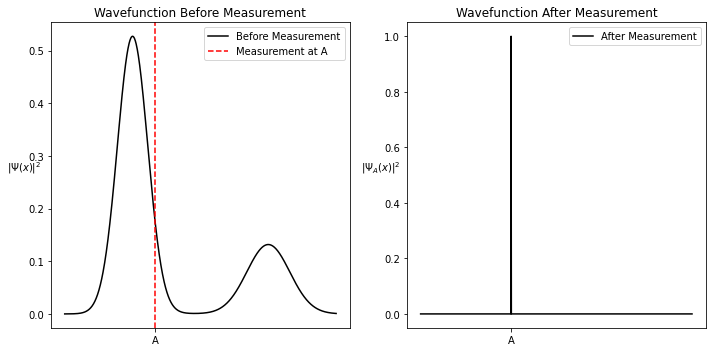
\includegraphics[scale=0.5]{collapseexample.png}
    \caption{An example of how a wave function collapses when a measurement is made at A.}
    \label{fig:collapse}
\end{figure}
\newline
This has quite fascinating implications for our world. That a simple interaction (ie. measurement) of a superposition of eigenstates can be reduced to a single eigenstate. Note that this is another way that a wave function might evolve. We already mentioned that a wave function may change with time, but it also changes when a measurement is made.
\subsubsection*{Postulate 4 - Expectation value}
If the state of the system is described by a normalised wave function $\Psi$, then the average (expectation) value of the observable corresponding to $\hat O$ is:
\begin{equation*}
    \langle \hat O \rangle = \int_{-\infty}^\infty \Psi^* \hat O \Psi d \tau
\end{equation*}
\subsubsection*{Postulate 5 - Time-Dependent Schrödinger Equation}
The wave function $\Psi$ of the system changes in time according to the time-dependent Schrödinger Equation:
\begin{equation*}
    H \Psi(r, t) = i \hbar \frac{\partial \Psi}{\partial t}
\end{equation*}
\subsubsection*{Postulate 6 - Anti-symmetry} \label{antisym}
The total wave function of a system of fermions (spin 1/2 particles) must be anti-symmetric with respect to the interchange of all coordinates of one particles with those of another.
\newline
This in turn gives rise to the Pauli exclusion principle, which is that two identical particles with half spins cannot occupy the same quantum state.
\section{The many-body problem}
Typically, in quantum mechanics we call a system of more than two particles a many-body system. The basis of this problem is that solving such systems accurately is a great challenge, and almost impossible to do analytically for large systems. \newline
If we consider first a classical system of $N$ particles, assume that it can move in three dimensions. It is normal to describe such a system using both it's position and velocity. For three dimensions that means that a total of $6$ values describe each particle. Ignoring any forces, the number of values used to describe such a system increases linearly with the amount of particles, $N \cdot \left(V + P\right)$ with $N$. Such a system, while maybe tedious and for very large $N$ computationally expensive, are still somewhat realistic to be able to solve, but let us now instead consider the quantum mechanical equivalent. \newline
In quantum mechanics such a system would instead be described as a superposition of the combinations of the single particle states. In this case, this results in a total of $\left(V + P\right)^N$ number of combinations. \newpage
It goes without saying that this is not feasible for many numbers of system, in fact, only a small minority are exactly solvable. We must therefore instead make use of approximations to solve the systems, of which there are many. Methods like the Hartree-Fock method, Full Configuration Interaction and of course, the Variational Monte Carlo. \newline
A natural extension for the Variational Monte Carlo method is of course to extend it to take advantage of machine learning. As we will see later in Sec. [\ref{nqs}], a neural network can approximate \textbf{any} function.
\section{The Variational Method} \label{varmethod}
But before we can move onto the Variational Monte Carlo, let us first study its 'forefather', the Variational Method. The Variational Method is a method in physics that enables us to solve problems using the calculus of variations or rather, variational calculus. The fundamental idea behind the variational method is that we can approximate some upper bound of a value, in our case the ground state energy $E_0$. In other words, we have some value $E_0$ we wish to find, which depends on some function $\psi$. By trying different $\psi$, we can get an estimate not only for what $\Psi$ may be, but also what $E_0$ may be. \newline
Let us for a moment assume a simple example. Assume that we have some Hamiltonian $H$ and a set of eigenvectors $\psi_\lambda$ such that
\begin{equation*}
    H | \psi_\lambda \rangle = \lambda | \psi_\lambda \rangle
\end{equation*}
and
\begin{equation*}
    \langle \psi_{\lambda_1} | \psi_{\lambda_2} \rangle = \delta_{\lambda_1 \lambda_2}
\end{equation*}
where $\delta_{ij}$ is the Kronecker delta:
\begin{equation*}
    \delta_{ij} = \begin{cases}
        0 & \text{if } i \neq j \\
        1 & \text{if } i = j
        \end{cases}
\end{equation*}
\newline If the lowest boundary of $H$ is $E_0$, then:
\begin{equation*}
    \langle \psi | H | \psi \rangle = \sum_{\lambda_1 \lambda_2} \langle \psi | \psi_{\lambda_1} \rangle  \langle \psi_{\lambda_1} | H | \psi_{\lambda_2} \rangle \langle \psi_{\lambda_2} | \psi \rangle
\end{equation*}
\begin{equation}
    \langle \psi | H |\psi \rangle = \sum_{\lambda} \lambda | \langle \psi_\lambda | \psi \rangle |^2 \geq \sum_\lambda E_0 | \langle \psi_\lambda | \psi \rangle |^2 = E_0 \langle \psi | \psi \rangle = E_0
\end{equation}
Here we see how we can use a $\psi$ to calculate some upper-bound for the ground state energy $E_0$. Ideally, as $\psi$ gets closer to the true wave function $\Psi$, $E_0$ should continuously decrease until we find a good approximation of $E_0$. That being said, we can never be sure how close we are to a true $E_0$, unless we of course know the analytical solution, but in that case what's the point?
\section{Trial Wave functions}
But how do we decide on what trial wave function to use? A trial wave function is, after all, just a normal function used as an ansatz. Typically, you'd want a function with as much overlap as possible with the true wave function. \newline
Let us call the trial wave function $\phi$, and the true wave function $\psi$. Assuming there is some overlap between $\psi$ and $\phi$, and $\phi$ is normalized such that:
\begin{equation*}
    \langle \phi | \phi \rangle = 1
\end{equation*}
then we wish to minimize the functional
\begin{equation*}
    E(\phi) = \langle \phi | H | \phi \rangle
\end{equation*}
This is however easier said than done. In many ways, in the variational method, finding a proper trial wave function is the biggest issue, so how do we find one?
\newline
Let us take a look at a relatively simple example. Consider the one dimensional harmonic oscillator described by the Hamiltonian
\begin{equation*}
    H = \frac{p^2}{2m} + \frac{1}{2} k x^2
\end{equation*}
Now, we of course know some physical properties of this hamiltonian, and typically you'd need atleast some knowledge of these to make some guess as to the shape of the wave function. \newline
We can make a reasonable guess that this Hamiltonian would have a Gaussian wave function, so let us try a few.
\newline
Let us make two guesses, first the exponential wave function $\phi_1$ and then later the Lorentzian wave function $\phi_2$ \cite{solveHO}
\begin{equation*}
    \phi_1 = A e^{-a |x|}
\end{equation*}
where A is the normalization constant and a is a real positive number.
\newline
First, we must find A.
\begin{equation*}
    \langle \phi_1 | \phi_1 \rangle = A^2 \int_{-\infty}^0 e^{2 a x} dx + A^2 \int_0^\infty e^{-2ax} dx
\end{equation*}
\begin{equation*}
    \langle \phi_1 | \phi_1\rangle = 2 A^2 \int_0^\infty e^{2 a x} dx = \frac{A^2}{a} \xrightarrow[]{} A = \sqrt{a}
\end{equation*}
The expectation value of H is then:
\begin{equation*}
    \langle \phi_1 | H | \phi_1 \rangle = \int_{-\infty}^\infty e^{-a |x|} \left( -\frac{\hbar^2}{2m} \frac{d^2}{dx^2} + \frac{1}{2} m \omega^2 A^2 x^2 \right) e^{-a |x|} dx
\end{equation*}
\begin{equation} \label{pluginphi1}
    \langle \phi_1 | H | \phi_1 \rangle = E_0 = \frac{m \omega^2}{4a^2} + \frac{\hbar^2 a^2}{2m}
\end{equation}
We must now minimize this expression with respect to $a$, which is:
\begin{equation*}
    \frac{\partial E_0}{\partial a} = 0 \xrightarrow[]{} \frac{\hbar^2 a}{m} - \frac{m \omega^2}{2a^3} = 0
\end{equation*}
\begin{equation*}
    a = \sqrt{\frac{m \omega}{\sqrt{2} \hbar}}
\end{equation*}
If we now use this $a$ in Eq. [\ref{pluginphi1}], we find:
\begin{equation} \label{phi1energy}
    E_0 = \frac{\hbar^2 m \omega}{2m \sqrt{2} \hbar} + \frac{m \omega^2 \sqrt{2} \hbar}{4 m \omega} = \frac{\hbar \omega}{\sqrt{2}} = 0.707\hbar\omega
\end{equation}
which, while okay, is still a $\sqrt{2}$ deviation from $E_0$, quite a significant margin when $E_0$ is so small. \newline
Let us now try $\phi_2$:
\begin{equation*}
    \phi_2 = \frac{A}{(1 + ax^2)^2}
\end{equation*}
\begin{equation*}
    \langle \phi_2 | \phi_2 \rangle = A^2 \int_{-\infty}^\infty \frac{1}{(1 + ax^2)^4} dx = A^2 \frac{5 \pi}{16 \sqrt{a}} \xrightarrow[]{} A = \sqrt{\frac{16 \sqrt{a}}{5\pi}}
\end{equation*}
We then solve same as before:
\begin{equation*}
    \langle \phi_2 | H | \phi_2 \rangle = A^2 \int_{-\infty}^\infty \frac{1}{(1 + ax^2)^2} \left( -\frac{\hbar^2}{2m} \frac{d^2}{dx^2} + \frac{1}{2} m \omega^2 A^2 x^2 \right) \frac{1}{(1 + ax^2)^2} dx
\end{equation*}
Which we solve as:
\begin{equation} \label{pluginphi2}
    \langle \phi_2 | H | \phi_2 \rangle = E_0 = \frac{7\hbar a}{10m} + \frac{m \omega^2}{10 a}
\end{equation}
\begin{equation*}
    \frac{\partial E}{\partial a} = 0 \xrightarrow[]{} \frac{7 \hbar^2}{10m} - \frac{m \omega^2}{10a^2} = 0
\end{equation*}
\begin{equation*}
    a = \frac{m\omega}{\sqrt{7} \hbar}
\end{equation*}
Plugging this $a$ into Eq. [\ref{pluginphi2}] gives:
\begin{equation}
    E_0 = \frac{7\hbar^2}{10m} \frac{m\omega}{\sqrt{7}\hbar} + \frac{m \omega^2}{10} \frac{\sqrt{7} \hbar}{m \omega} = \frac{\sqrt{7} \hbar \omega}{5} = 0.529\hbar \omega
\end{equation}
which is only a $\sqrt{7}/5$ deviation from $E_0$. \newline
Here we see clearly how much of a difference a good ansatz makes. $\phi_1$ deviated by $41.4\%$ whereas $\phi_2$ deviated with only $5.80\%$. We can further see this illustrated in the figure below:
\begin{figure}[ht!]
    \centering
    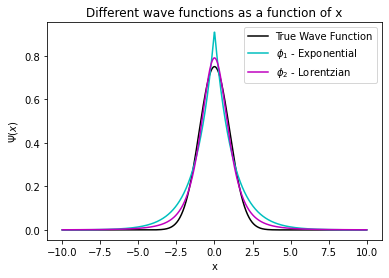
\includegraphics[scale=0.5]{HOexample.png}
    \caption{Here we see clearly how despite the wave functions ultimately being very alike to the true wave function, even small margins in overlap can give wildly different estimations of $E_0$}
    \label{figHOs}
\end{figure}
\section{The Variational Monte Carlo}
The Variatonal Monte Carlo (VMC) is an extension of the variational principle. It combines the variational principle with Monte Carlo integration and a sampling method to determine (in our case) an estimation of the upper-bound of a ground state energy. Given some system of particle $N$ in $M$ dimensions require an integral of $N \times M$ dimensions, which is intractable for most cases. To see why, consider again:
\begin{equation*}
    E_0 = \leq \frac{\langle \psi| H | \psi \rangle}{\langle \psi | \psi \rangle} = E
\end{equation*}
If we were to evaluate this for a system of size $N \times M$, we have:
\begin{equation} \label{tosolve}
    E = \frac{\int \psi^*(r) H \psi (r) dr}{\int \psi^* (r) \psi (r) dr}
\end{equation}
where r is a set of all particle coordinates $r = (r_1, r_2, \dots, r_N$ \newline
It is quite obvious why such systems are intractable to solve when they are large, instead, we must approximate. One such way of approximating is by sampling, as the success of the Monte Carlo integration depends directly on the quality (and number) of samples.\newline
\subsection{Monte Carlo integration}
Monte Carlo integration is the idea that we use random numbers to evaluate some integral numerically. In our case, this would be to evaluate energy, wherein the numbers used are drawn from the probability distribution associated with the energy. \newline
To give an example of this in practice, consider a box of dimensions $L, M, N$. Calculating the volume of such a box is trivial, of course, it is given by:
\begin{equation*}
    V = \int_{n_1}^{n_2}\int_{m_1}^{m_2}\int_{l_1}^{l_2} 1 dl \; dm \; dn 
\end{equation*}
Now, imagine we had a weird, indescribable shape inside. Exactly what kind of shape you imagine doesn't really matter, but it needs to be hard to describe with a volumetric integral. Imagine now we place some $K$ number of dots inside if we know that the volume of the box is $V$, then would the percentage of dots $K$ inside the odd shape not be a good indicator of its volume, provided the samples drawn are good? \newline
In other words, and perhaps a bit more relevant, we want to evaluate:
\begin{equation*}
    \langle E \rangle = \int_{-\infty}^\infty dx P(x) E(x)
\end{equation*}
which gives us the approximation:
\begin{equation*}
    \langle E \rangle = \int_{-\infty}^\infty dx P(x) E(x) \approx \frac{1}{N_{mc}} \sum_{i=1}^{N_{mc}} E(x_i)
\end{equation*}
where $N_{mc}$ are the number of Monte Carlo cycles, ie. how many times we let the algorithm run. The values $x_i$ are sampled from the probability distribution of $P(x)$, and this actually gives us a good approximation of the integral Eq. [\ref{tosolve}]. \newline
If we know ahead of time sort of what the distribution $P(x)$ looks like, then, provided our samples are initialized accordingly, we may not need that many cycles to reach a sufficient approximation. If, however, we do not know the distribution, then we may need many cycles until the samples are sufficiently like the distribution $P(x)$. It is therefore important that we choose a good sampling method, of which there are many. Let us take a look at some now:
\subsection{Sampling} \label{metro}
We first introduce a very simple method of sampling. Assume we have a vector of positions $r$. We select then a random value $i$ and update the position as:
\begin{equation*}
    r_{n} = r_i + \delta p
\end{equation*}
where $\delta$ is a step-size and $p$ is a uniform distribution in the interval $[-1, 1]$. The acceptance probability is then given by:
\begin{equation*}
    A = \text{min}\left(1, \frac{|\Psi(r_i)|^2}{|\Psi(r_n)|^2}\right)
\end{equation*}
which is the probability that the move will be accepted. \newline
This is the 'brute-force' method, or the Metropolis method, but we can improve it by introducing a bit more nuance to the algorithm.
\newline
First, we start by introducing a quantum force term, given by:
\begin{equation*}
    F = \frac{2}{\Psi}\nabla \Psi
\end{equation*}
This is also called the drift term, and why that is can be seen for the modified proposed new positions:
\begin{equation*}
    r_n = r_i + \sqrt{\delta}P + D F \delta
\end{equation*}
here, we have the same term as above, but the probability distribution is now Gaussian as opposed to uniform. We also introduce the new quantum force term, with a diffusion constant $D$ (typically 0.5).
\newline
We also use this force to calculate Green's function as:
\begin{equation*}
    G = \frac{1}{(4\pi D \delta)^{3N/2}} \times \exp \left(-\frac{(r_n - r_i - D \delta F_i)^2}{4\pi D \delta}\right)
\end{equation*}
which we use to modify the calculation of the acceptance probability:
\begin{equation*}
    A = \text{min} \left( 1, \frac{G|\Psi(r_i)|^2}{G|\Psi(r_n)|^2}\right)
\end{equation*}

This method is an extension of the Metropolis method, called the Metropolis-Hastings method, and is the method we'll be using for continuous systems. \newline
In the case of a binary or quantized system (where values are not continuous), we cannot calculate a quantum force nor the resulting Green's function. Consider a system of spins on a one-dimensional lattice of length $L$. The only action such a system can take is flipping it's spin, so we then instead get:
\begin{equation*}
    r_n = -r_i
\end{equation*}
where the acceptance probability is evaluated same as in the brute-force method.
\newline
An example of the metropolis-hastings algorithm in action can be seen below.
\begin{figure}[ht!]
    \centering
    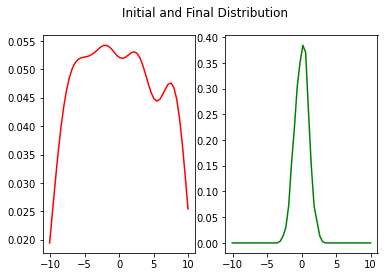
\includegraphics[scale=0.5]{MHexample.png}
    \caption{An example of how the Metropolis-Hastings algorithm helps shape our samples to more correctly fit the target probability distribution decided by the wave function. Here for 1000 samples over 300 iterations.}
    \label{fig:mh}
\end{figure}
\newline
Here, we started with an initial uniform distribution on the span $[-10, 10]$, and over 300 iterations we see how the distribution moves to be more in line with the targeted Gaussian distribution.
\newpage
\section{Hebbian Theory}
We mentioned it briefly in the introduction, but let us give a brief introduction to Hebbian theory, in many ways one of the bases of neural networks. You may recall from Sec. [\ref{hebbcite}] that \newline
\textit{\textcolor{direct-cite}{When an axon of cell A is near enough to
excite a cell B and repeatedly or persistently takes part in firing it, some growth process or metabolic
change takes place in one or both cells such that A’s efficiency, as one of the cells firing B, is increased.’}} \newline
If we assume a unit of a neural network to correspond to a neuron, such that the $i$-th neuron is described by $\boldsymbol{X}_i$, we can model a theoretical neural network by as a set of connections between the different neurons $\boldsymbol{X}_i, \boldsymbol{X}_{i+1}$ etc.. In accordance with the citation above, if some neuron $i$ and $j$ fire together, their associated weight $w_{ij}$ is increased, thus strengthening their connection. The increase in those weights are however not linear. Indeed, if neuron $i$ and $j$ are expected to fire together, then a common firing of $i$ and $j$ has a minuscule effect on their associated weight $w_{ij}$. Likewise, if neuron $i$ and $j$ are expected to fire together but they don't, we will see a reduction to their associated weights. \newline
How exactly the weights are updated is decided by two factors. One, the optimizer/learning-rule we're using for our particular model and two, the loss or cost function
\subsection{Optimizers} \label{opt}
An optimizer is another word for the algorithm we're going to be using to update the weights of our networks. Typically this is done by a family of methods called gradient-descent methods. As the name may suggest, the method takes the gradients of the function with respect to the parameters, and tries to update the parameters such that we reach a local minima. \newline Imagine if you will that you were dropped on a bumpy (but safe) series of hills with a blindfold on and told to get off the mountain. Naturally you'd be inclined to follow the slope downwards. The gradient descent methods work much the same way. The landscape of the loss function spans a series of hills and valleys, and we want to find the lowest most point.
\newline
Let us examine the simplest possible gradient descent method:
\begin{equation*}
    \theta = \theta - \eta \nabla_\theta \mathcal{E}(\theta)
\end{equation*}
Here, $\theta$ are the parameters with which we optimize the loss function $\mathcal{E}$. The learning rate, typically denoted by $\eta$ is the degree with which we update the parameter $\theta$. $\nabla_\theta$ is the gradient of the loss function with respect to the parameter $\theta$, but it needs to do this for the entire dataset, every step. It goes without saying that for any respectable data set, this will be very slow, so we will need to further iterate and improve the method, although it is worth mentioning that the regular gradient descent method will always converge to the global minimum for convex loss function landscapes, and local minima for non-convex loss function landscapes.
\newline
We introduce the stochastic gradient descent method, as:
\begin{equation*}
    \theta = \theta - \eta \nabla_\theta \mathcal{E}(\theta; x^{(i)}; y^{(i)})
\end{equation*}
which is similar to that of the regular gradient descent, but now instead updates the parameter for each sample $x^{(i)}$ and corresponding target $y^{(i)}$. This solves the issue of the computation time of the regular gradient descent. This results in a high variance, and we can thus even jump out of local minima 'valleys' which regular gradient descent was not able to. This also means that it is susceptible to overshooting local or global minima, making convergence time.
\newline
We choose then instead to batch our data, as this will help both reducing the variance of our parameter $\theta$, but also allow us to take advantage of matrix computation. This 'mini-batch' gradient descent method then takes the shape of:
\begin{equation*}
    \theta = \theta - \eta \nabla_\theta \mathcal{E}(\theta; x^{(i:i+n)}; y^{(i:i+n)})
\end{equation*}
where $(i:i+n)$ are the batched values, of length $n$. Note that the 'stochastic' name of these method comes from the fact that we shuffle the data set for every epoch. For simplicity's sake, we will from now on refer to the 'mini-batch' gradient descent as SGD.
\newline
We now have a good baseline, but this method is still insufficient for difficult error-landscapes, something extremely common for neural networks. We need to tackle a few difficulties the SGD method has, notably, and perhaps most importantly its tendency to get 'stuck' in local suboptimal minima.
\newline
Imagine if you will that you find yourself in a 'ravine'. The ravine just barely trends downwards to the ground-level, flanked by two steep cliffs on each side. Using our SGD method as is, it is likely that we'd find ourselves ping-ponging between the steep gradients formed by the cliffs, making little to no progress towards the actual ground-level at the end of the ravine. One way to remedy this is to add a momentum term, a term that strengthens the contributions of the gradients repeatedly pointing the same direction, and weakens the contribution of the gradients pointing in the opposite direction. This takes the form of:
\begin{equation*}
    v_t = \gamma v_{t-1} + \eta \nabla_\theta \mathcal{E}(\theta; x^{(i:i+n)}; y^{(i:i+n)})
\end{equation*}
\begin{equation*}
    \theta = \theta - v_t
\end{equation*}
We see here that the term $v_t$ retains some information from it's previous iteration $v_{t-1}$, and that its strength is decided by a momentum parameter $\gamma$. The momentum term $v_t$ is actually a moving average over the recent gradients and the term $\gamma$ effectively decides for how long to store the previous gradients. This reduces the oscillation of our movement toward the minima, and also provides faster convergence.
\newline
Let us now take a small detour. One issue with the methods above is that the learning rate $\eta$ is static. This leads to a situation where the updates made parameter $\theta$ may overshoot or undershoot depending on the situation. If we have a very small $\eta$, we may find that convergence takes a very long time, but when we finally do converge, we don't run the risk of overshooting. This of course also means that it'll be harder to escape local minima. The opposite is also an issue, for a large $\eta$, we will see fast convergence, but we will have a problem with reaching the exact minima, continuously overshooting as we oscillate over the minima. \newline
What if we could introduce a method that has a adaptive learning rate? Adagrad is such a method, and it is:
\begin{equation*}
    g_{t,i} = \nabla_{\theta_t} \mathcal{E}(\theta; x^{(i:i+n)}; y^{(i:i+n)})
\end{equation*}
where $g_{t,i}$ is the gradient of the loss function with respect to the parameter $\theta_i$ and step $t$. We then have:
\begin{equation*}
    \theta_{t+1, i} = \theta_{t,i} - \eta g_{t,i}
\end{equation*}
We are now missing just one term that scales $\eta$ as advertised, and this is:
\begin{equation*}
    \theta_{t+1, i} = \theta_{t,i} - \frac{\eta}{\sqrt{G_{t, ii} + \epsilon}} g_{t,i}
\end{equation*}
where $\epsilon$ is a smoothing term to avoid division by zero, and $G$ is a diagonal matrix where the diagonal elements is the sum of squares with respect to $\theta_i$ up to time step $t$. \newline
This method is fine, however the gradients accumulated in the denominator causes $\eta$ to become very small, and thus leads to vanishing gradients.
\newline A method proposed to remedy this is RMSprop. We employ a running average $E[g^2]_t$ at step $t$ that then depends on the previous average and the current gradient, as:
\begin{equation*}
    E[g^2]_t = \gamma E[g^2]_{t-1} + (1 - \gamma)g^2_t
\end{equation*}
If we instead let this be the denominator for $\eta$, we find
\begin{equation*}
    \theta_{t+1} = \theta_t - \frac{\eta}{\sqrt{E[g^2]_t + \epsilon}} g_t
\end{equation*}
The learning rate is divided by an exponentially decaying average of squared gradients, giving us the adaptive learning rate we desired.
\newline
There's one last thing to discuss. Typically, a method called Adam, is described as RMSprop with momentum, essentially combining the best of both worlds. We calculate the exponentially decaying average of past gradients (like momentum) as $m_t$ and the exponentially decaying average of past squared gradients (like RMSprop) as $v_t$ and giving:
\begin{equation*}
    m_t = \beta_1 m_{t-1} + (1 - \beta_1)g_t
\end{equation*}
\begin{equation*}
    v_t = \beta_2 v_{t-1} + (1 - \beta_2) g^2_t
\end{equation*}
$m_t$ and $v_t$ are then the estimates of the first and second moment of the gradients respectively, giving it its name ADAptive Moment estimation, ADAM. We initialize $m_t$, $v_t$ as vectors of 0s, biasing them towards zero, which we counteract by accounting for the bias:
\begin{equation*}
    \hat m_t = \frac{m_t}{1 - \beta_1^t}
\end{equation*}
\begin{equation*}
    \hat v_t = \frac{v_t}{1 - \beta_2^t}
\end{equation*}
Finally giving us the update rule for Adam:
\begin{equation}
    \theta_{t+1} = \theta_t - \frac{\eta}{\sqrt{\hat v_t} + \epsilon}\hat m_t
\end{equation}
which is what we'll be using
\subsection{The loss function} \label{losssec}
We now move on to the other piece of the puzzle for training our network, the loss function. Naturally, we cannot use a regular loss function here, like the mean-squared-error or cross-entropy as we have no target, we do not know what the ground-state energy is for most systems, and even if we did it defeats the purpose of the network as a substitute for the wave function. However, in practice a loss function is really just a function to be minimized. Since we know that $E_0$ is lower-bounded as described in Sec. [\ref{varmethod}], we can use the estimation of the energy as a substitute for our loss function. 
\newline The expectation energy of a system is defined as:
\begin{equation*}
    \langle E \rangle = \frac{\langle \psi | \hat H | \psi \rangle}{\langle \psi | \psi \rangle}
\end{equation*}
for a wave function $\psi$ and hamiltonian $\hat H$
\newline
We rewrite this as:
\begin{equation*}
    \langle E \rangle = \frac{\int \psi^* (x) \hat H \psi(x) dx}{\int \psi^*(x) \psi(x) dx}
\end{equation*}
\begin{equation*}
    \langle E \rangle = \frac{\int \psi^* (x) \left(\psi(x) \frac{1}{\psi(x)} \right) \hat H \psi(x) dx}{\int | \psi(x)|^2 dx}
\end{equation*}
\begin{equation*}
    \langle E \rangle = \frac{\int \psi^* (x) \psi(x) \left(\frac{\hat H \psi(x)}{\psi(x)}\right) dx}{\int | \psi(x)|^2 dx}
\end{equation*}
Note the term $\left(\frac{\hat H \psi(x)}{\psi(x)}\right)$. This term is typically called the local energy $E_L$, and we will use it to as the quantity to be minimized. We write further:
\begin{equation} \label{loss}
    E_0 \approx \frac{1}{N} \sum_{i=1}^N E_L(x)
\end{equation}
where $E_L$ is evaluated for coordinates $x$ randomly samples from the probability distribution of the wave function $\psi$, $|\psi|^2$.
\newline
Note that this isn't necessarily exclusive to the energy. This can be done for any observable, so a more general form would be
\begin{equation*}
    O_L \approx \frac{1}{N}\sum_{i=1}^N O_L(x)
\end{equation*}
to evaluate any local observable, but for this work we will stick to just the energy.
\newline
Although we won't need to calculate the gradients by hand, given the auto-differentiation of the libraries Jax and PyTorch (see Sec. [\ref{Jax}], Sec. [\ref{PyTorch}]), we should still derive them, if only to make sure our model is correct.
\newline
We have first the local energy give by:
\begin{equation*}
    E_L = \frac{\hat H \psi(x)}{\psi(x)}
\end{equation*}
with the associated gradient
\begin{equation} \label{lossgrads}
    g_i = \frac{\partial \langle E_L \rangle}{\partial w_i} = 2\left( \left\langle E_L \frac{1}{\psi} \frac{\partial \psi}{\partial w_i} \right\rangle - \langle E_L \rangle \left\langle \frac{1}{\psi} \frac{\partial \psi}{\partial w_i} \right\rangle \right)
\end{equation}
where $w$ are the weights of our network.
\newline
\section{The Neural Quantum State} \label{nqs}
In the grand scheme of things, using a neural network to represent the wave function is a pretty new concept\cite{NQS}, the idea being that you treat the neural network as a 'black box', such that for an input $\mathcal{X}$, it returns amplitudes in accordance with $\Psi(\mathcal{X})$. We know this is possible because of the universal approximation theorem, which states that for any arbitrary function $\mathcal{F}$, there is a neural network that can approximate that function. This is done by modifying the weights associated with each node of the neural network, of which there are many, increasing exponentially as we increase the depth of the network. The depth refers to how many hidden layers the neural network has. Typically, a network is referred to as deep if it has more than one hidden layer, and as we increase the depth, the network becomes more complex and better fit to tackle complex systems. 
\newline
\subsection{Neural Networks}
Let us first tackle Neural Networks in the context of a neural quantum state:
\subsubsection{Forward pass}
Let us for a moment consider the simplest model of a Neural Network, the perceptron \cite{NN1969}. Consider a system of $M$ inputs, the perceptron would then be:
\begin{figure}[ht!]
    \centering
    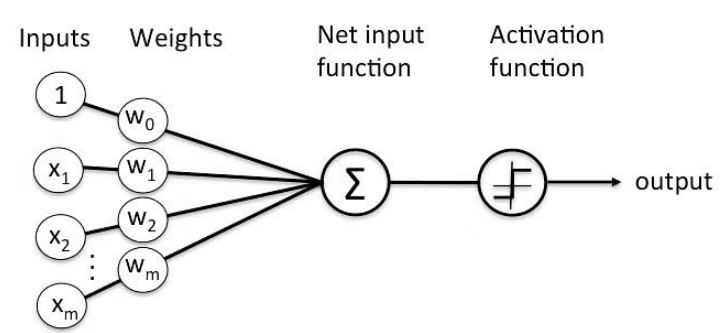
\includegraphics[scale=0.5]{perceptron.PNG}
    \caption{An illustration of a perceptron, a grandfather of neural networks. Note the constant term (or bias) as the uppermost input. This serves to shift the activation funciton
    \newline \href{https://arxiv.org/pdf/1708.06008}{Image Source}
    }
    \label{fig:perceptron}
\end{figure}
\newline
Here, we simply multiply each of the inputs $x_i$ with their associated weights $w_i$ and sum them, before they are passed through the activation function, giving us the output. This is such that for some activation function $a(x)$, we may write the output as:
\begin{equation*}
    y = a(x w)
\end{equation*}
Note that we can write the multiplication and summation of $x_i$ and $w_i$ as an inner product.
\newline
Let us now try to add more layers, so we can see how data is passed through the neural network. We will introduce some notation. We denote weights as: $w_{i}^{(j)}$ which is the i'th weight on the j'th layer, such that the output of layer 1 may be written as:
\begin{equation*}
    y_i^{(1)} = a \left( \sum_{i}^{N^{(0)} + 1} x_i w_{ij}^{(0)} \right)
\end{equation*}
where $N^{(0)}$ is the number of units in layer 0. \newline
Here, we calculate the output of layer 0 (ie. the input to layer one, $y_i^{(1)}$) using the weights and inputs. Note that we have to add a +1 to the summation, because we also have the constant (bias) term and its weights. \newline
If we then let $x_i = y_i^{(0)}$, we can write this more generally as:
\begin{equation} \label{output}
    y_i^{(j+1)} = a \left(\sum_{i}^{N^{(j)} + 1} y_i^{(j)} w_{ij}^{(j)} \right)
\end{equation}
\subsubsection{Backward propagation}
Backward propagation is what we use to optimize the weights of the neural network. It is one of the most common means of training a network. The means of training is that we calculate the gradient of the chosen loss function with respect to the weights $w$ of the network. \newline 
Assume we have some neural network with $L$ layers, an input $x$ and a corresponding output $y$. The backpropagation method is four distinct steps. First, we compute the forward pass as above, until we have an output $y$.
\newline
Let us rewrite Eq. [\ref{output}] by naming the contents being passed to the activation function $a$ as $k$.\newline If so, then:
\begin{equation*}
    k_i^{(j)} = \sum_i^{N^{(j)} + 1} y_i^{(j)} w_{ij}^{(j)}
\end{equation*}
such that:
\begin{equation*}
    y_i^{(j+1)} = a(k_i^(j))
\end{equation*}
The second step is typically to use the neural network to calculate whatever value $f(y)$ we wish to, in our case, this would be the local energy. However, as we have no true traditional loss function, this local energy also becomes the loss function. This provides a unique situation where the loss function itself is what we wish to calculate. The second step, which is calculating the target $f(y)$ and the third step, which is using that $f(y)$ to calculate the loss, are then merged as one single step. The loss function, as we know is:
\begin{equation*}
    \mathcal{L} = \frac{1}{N} \sum_{i=1}^N E_L(x; w)
\end{equation*}
where
\begin{equation*}
    E_L(x; w) = \frac{1}{\psi(x, w)} H\psi(x; w)
\end{equation*}
and $x$ are the inputs whilst $w$ are the weights. After computing the loss $\mathcal{L}$, we lastly get to the final fourth step, the backward pass from which backpropagation gets its name. We now need to calculate the gradient of $\mathcal{L}$ with respect to the parameters $w$. As the name suggests, we need to start from the back, first, we calculate the gradient with respect to the output:
\begin{equation*}
    \frac{\partial \mathcal{L}}{\partial y_i^{(L)}}  = \frac{\partial \mathcal{L}}{\partial E_L}  \frac{\partial E_L}{\partial y_i^{(L)}} 
\end{equation*}
We then calculate the gradients of the loss function with respect to $k_i^{(j)}$, which is:
\begin{equation*}
    \frac{\partial \mathcal{L}}{\partial k_i^{(j)}} = \frac{\partial \mathcal{L}}{\partial y_i^{(j+1)}}  \frac{\partial y_i^{(j+1)}}{\partial k_i^{(j)}}  = \frac{\partial a'(k_i^{(j)})}{\partial y_i^{(j+1)}} 
\end{equation*}
where $a'$ is the derivative of the activation function with respect to $k_i^{(j)}$.\newline
We can now finally express the loss gradient with respect to the weights $w_{ij}^{(j)}$, which is:
\begin{equation*}
    \frac{\partial \mathcal{L}}{\partial w_{ij}^{(j)}} = \frac{\partial \mathcal{L}}{\partial k_i^{(j)}}  \frac{\partial k_i^{(j)}}{\partial w_{ij}^{(j)}}  = \frac{\partial \mathcal{L}}{\partial k_i^{(j)}}  y_j^{(j)}
\end{equation*}
which we then use to update our weights using our chosen optimizer, ADAM.
\subsubsection{Activation functions}
We've mentioned activation functions a fair bit without necessarily going too much into detail about what they are, so it's only natural we now discuss them. The primary goal of the activation functions is to introduce non-linearity to the output of a node. The activation functions are thus one of the most important components of the neural network, as it is one of its main strengths, as it allows us to capture intricate patterns in the data that normal linear models are unable to. \newline
The most common activation function is that of the Sigmoid function, given by:
\begin{equation*}
    a_{sigmoid}(x) = \frac{1}{1 + e^{-x}} 
\end{equation*}
which is fine, but has since been replaced by newer and better activation functions. Another thing we need to keep in mind is that these are not only to be used in the backpropagation to calculate the gradients with respect to the weights, but the activation functions will also play a central role in the calculations of the gradients of $\psi(x)$ with respect to $x$. As such, it is important to not select an activation function that does not suffer from vanishing gradients. This means that both the Sigmoid function and the hyperbolic tangent, as these both suffer from vanishing gradients for low and high inputs respectively. \newline 
One of the simplest, computationally efficient and popular activation functions is that of the Rectified Linear Unit, or ReLU, which is defined as:
\begin{equation*}
    a_{ReLU} = \text{max}(0, x)
\end{equation*}
As you can see, this output is strictly positive and linear. This is fine for most purposes but poses a problem. That is, for strictly positive activation functions, it is impossible for the wave function to be anti-symmetric without manually ensuring it \cite{symm}. ReLU also runs the risk of nodes permanently deactivating if they continuously output zero, dubbed the 'dying ReLU' problem \cite{dying}, thus resulting in that neuron outputting $0$ for any input $x$. We must also keep in mind that ReLU is poorly defined for complex inputs, which can happen, so if necessary we can build a custom ReLU in accordance with \cite{cnn}, which suggests a phase-amplitude activation as:
\begin{equation*}
    a_{cReLU} = a_{ReLU}(|x|) \cdot e^{i \theta_x}
\end{equation*}
where $\theta_x$ is the angle in radians for the input $x$. This way we can still use ReLU for complex-valued inputs, to keep our network at least somewhat consistent.
\newline
\subsection{Restricted Boltzmann Machines} \label{RBM}
We now move onto the RBM.
\subsubsection{Boltzmann Machines}
Before we go into Restricted Boltzmann Machines (RBMs), it may be beneficial to first mention regular Boltzmann Machines (BMs). A Boltzmann Machine is an undirected probabilistic graphical (and generative) model with stochastic continuous or discrete units. \newline
\begin{figure}[ht!]
    \centering
    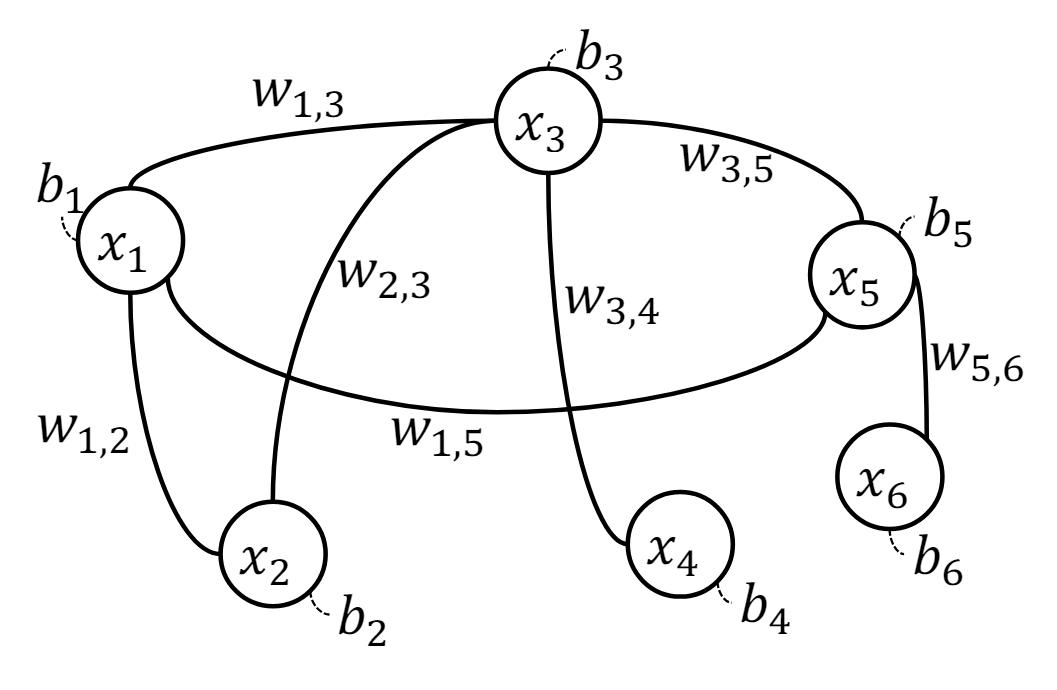
\includegraphics[scale=0.3]{BM.PNG}
    \caption{An illustrative Boltzmann machine
    \newline
    \href{https://arxiv.org/pdf/1708.06008}{Image Source}
    }
    \label{fig:BM}
\end{figure} \newline
The Boltzmann machine is a network where each pair of units $n$ is connected by an edge. This means that the Boltzmann machine is a fully connected network. There are two types of nodes, they are either visible units $v$ or hidden units $h$. The visible nodes are typically the dimension of the data, so two particles in two dimensions would mean four visible units. The hidden units are feature extractors, and serve to find hidden correlations and interactions between the visible nodes. Thus the more hidden units, the more complex the network.
\newline
Typically, these networks have a quantity associated with them called the energy, and it is given by \cite{mhjorth-RBM}:
\begin{equation*}
\begin{split}
    E(v, h) = - \sum_{i,k}^{M,K} a_i^k \alpha_i^k (v_i) - \sum_{j, l}^{N, L} b_j^l \beta_j^l (h_j) - \sum_{i,j,k,l}^{M,N,K,L} \alpha_i^k (v_i) w_{ij}^{kl} \beta_j^l (h_j) \\
    - \sum_{i,m=i+1, k}^{MM, K} \alpha_i (v_i) x_{im}^k \alpha_m^k (v_m) - \sum_{j,n=j+1, l}^{N,N,L} \beta_j^l (h_j) y_{jn}^l \beta_{n}^l (h_n)
\end{split}
\end{equation*}
\newline
This equation warrants some explanation. $\alpha^k_i (v_i)$ and $\beta^l_j (h_j)$ are one dimensional transfer functions from the input to the feature value. They are unaffected by the training of the model (ie. they are constant as the training parameters change). Labels $k, l$ denote that there are more than one transfer function per variable.
\newline
We can then represent the wave function by the marginal probability distribution:
\begin{equation*}
    P(v, h) = \frac{1}{Z} e^{-\frac{1}{T_0} E(v, h)}
\end{equation*}
where $T_0$ is typically ignored by setting it to one. Z is the partition function and is given as:
\begin{equation*}
    Z = \int \int e^{-\frac{1}{T_0} E(v, h)}
\end{equation*}
\newline
The Boltzmann machine is hard to train, but if we were to restrict the intra-layer connections $x, y$ of the energy function $E(v, h)$, we end up with the Restricted Boltzmann Machine, RBM.
\subsubsection{Restricted Boltzmann Machines}
The RBM differs from the BM in that there are no lateral connections between the visible nodes, nor are there any lateral connections between the hidden nodes. We can thus get the new energy function by setting these intra-layer connections to 0, giving:
\begin{equation*}
    \begin{split}
    E(v, h) = - \sum_{i,k}^{M,K} a_i^k \alpha_i^k (v_i) - \sum_{j, l}^{N, L} b_j^l \beta_j^l (h_j) - \sum_{i,j,k,l}^{M,N,K,L} \alpha_i^k (v_i) w_{ij}^{kl} \beta_j^l (h_j) \\
    - 0\sum_{i,m=i+1, k}^{MM, K} \alpha_i (v_i) \alpha_m^k (v_m) - 0\sum_{j,n=j+1, l}^{N,N,L} \beta_j^l (h_j) \beta_{n}^l (h_n)
\end{split}
\end{equation*}
\begin{equation*}
    E(v, h) = - \sum_{i,k}^{M,K} a_i^k \alpha_i^k (v_i) - \sum_{j, l}^{N, L} b_j^l \beta_j^l (h_j) - \sum_{i,j,k,l}^{M,N,K,L} \alpha_i^k (v_i) w_{ij}^{kl} \beta_j^l (h_j)
\end{equation*}
The exact form of the energy function from here depends on what type of RBM we're dealing with. Let us consider the two most common forms of RBM.
\newline
First, the binary-binary RBM, which takes the form:
\begin{equation*}
    E(v, h) = - \sum_i^M v_i a_i - \sum_j^N b_j h_j - \sum_{i,j}^{M,N} x_i w_{ij}h_j
\end{equation*}
Here, the vectors $v$ and $h$ are both entirely binary, typically values 0 and 1.
\newline
Another common form is the gaussian-binary RBM, which is:
\begin{equation*}
    E(v, h) = - \sum_i^M \frac{(v_i - a_i)^2}{2 \sigma_i^2} - \sum_j^N b_j h_j - \sum_{i,j}^{M,N}  \frac{x_i w_{ij}h_j}{\sigma_i^2}
\end{equation*}
Here $v$ is gaussian while $h$ is binary.
\newline
Both RBMs serve different purposes, and which one we find best depends on the system we're studying. For example, if you're studying a harmonic oscillator, it would make sense for the positional vector $v$ to be gaussian, but if you're studying a system of latticed spins where the spins take on a binary value of $s = \pm \frac{1}{2}$, it may be more beneficial to use the binary-binary RBM.
\newpage
~\newpage
\part{Method}
\section{Representing the wave function}
Let us now move on to how we may use our neural network architectures to solve quantum mechanical systems. We're going to do this by using the architectures to represent the wave function, the method which we use to do so depending on the architecture used.
\subsection{Restricted Boltzmann Machine}
In the case of the RBM, we may represent the wave function as the marginal probability distribution\cite{mhjorth-RBM}. \newline Recall that:
\begin{equation} \label{proba}
    P(x, h) = \frac{1}{Z} e^{- \frac{1}{T_0} E(x, h)}
\end{equation}
where Z is a normalization constant defined as:
\begin{equation} \label{part}
    Z = \int \int e^{- \frac{1}{T_0} E(x, h)} dxdh
\end{equation}
where $T_0$ is typically set to 1.
\newline Note that $E$ is dependent on the type of RBM discussed in Sec. [\ref{RBM}]
\newline We now rewrite Eq. [\ref{proba}] such that $P$ depends only on $\mathbf{x}$, giving us the marginal probability:
\begin{equation*}
    F(x) = \sum_h P(x, h) = \frac{1}{Z} \sum_h e^{-E(x, h)}
\end{equation*}
we now rename this to $\Psi$, such that:
\begin{equation*}
    \Psi(x) = F_{rbm}(x) = \frac{1}{Z} \sum_h e^{-E(x, h)}
\end{equation*} 
\begin{equation*}
    \Psi(x) = \frac{1}{Z} \sum_{h_j} \exp\left(-\sum_i^M \frac{(x_i-a_i)^2}{2\sigma^2} + \sum_j^N b_j h_j + \sum_{ i,j}^{M,N} \frac{x_i W_{ij} h_j}{\sigma^2} \right)
\end{equation*}
finally giving:
\begin{equation}
    \Psi(x) = \frac{1}{Z} e^{-\sum_i^N \frac{(x_i - a_i)^2}{2\sigma^2}} \prod_j^N \left(1 + e^{b_j + \sum_i^M \frac{x_i W_{ij}}{\sigma^2}} \right)
\end{equation}
And while this wave function is fine, it is considered a more general one because it allows for complex valued wave functions, but it also means that the probability of the RBM is now an amplitude, thus changing the probabilistic foundation of the RBM. This causes a lot of the surrounding theoretical framework to break down. If we instead assume the wave function to be positive definite we can use the RBM to represent the squared wave function, and thus a probability. Thus we have:
\begin{equation*}
    | \Psi(x)|^2 = F(x)
\end{equation*}
\begin{equation}
    \Psi(x) = \sqrt{F} = \frac{1}{\sqrt{Z}} e^{-\sum_i^N \frac{(x_i - a_i)^2}{4\sigma^2}} \prod_j^N \sqrt{1 + e^{b_j + \sum_i^M \frac{x_i W_{ij}}{\sigma^2}}}
\end{equation}
Previously, we showed explicitly the gradients of the weights with respect to the loss function for the Neural Network model. However, we neglected to do so for RBM, as we did not yet have an expression for the wave function. Now that we have the expression above, let us now find these explicit gradients. \newline
Recall Eq. [\ref{lossgrads}]. We can now use the energy term of the RBM to more explicitly define the gradient calculation for $a_i$, $b_j$ and $w_{ij}$ respectively.
\newline
We use that $\frac{1}{\Psi} \frac{\partial \Psi}{\partial w_i} = \frac{\partial \ln \Psi}{\partial w_i}$ and find:
\begin{equation*}
    \ln \Psi (x) = - \ln Z - \sum_m^M \frac{(x_m - a_m)^2}{2 \sigma^2} + \sum_n^N \ln \left(1 + \exp\left(b_n + \sum_i^M \frac{x_i w_{in}}{\sigma^2}\right)\right)
\end{equation*}
giving:
\begin{equation*}
    \frac{\partial}{\partial a_m} \ln \Psi = \frac{1}{\sigma^2} (x_m - a_m)
\end{equation*}
\begin{equation*}
    \frac{\partial}{\partial b_n} \ln \Psi \frac{1}{e^{-b_n - \frac{1}{sigma^2}\sum_i^M x_i w_{in}} + 1}
\end{equation*}
\begin{equation*}
    \frac{\partial}{\partial w_{mn}} \ln \Psi = \frac{x_m}{\sigma^2\left(e^{-b_n - \frac{1}{sigma^2}\sum_i^M x_i w_{in}} + 1\right)}
\end{equation*}
using then the definition of $\Psi$, we get:
\begin{equation*}
    \ln \Psi = - \frac{1}{2} \ln Z - \sum_m^M \frac{(x - a_m)^2}{4\sigma^2} + \frac{1}{2} \sum_n^N \ln \left( 1 + \exp\left(b_n + \sum_i^M \frac{x_i w_im}{\sigma^2}\right)\right)
\end{equation*}
giving us finally:
\begin{equation}
    \frac{\partial}{\partial a_m} \ln \Psi = \frac{1}{2 \sigma^2} (x_m - a_m)
\end{equation}
\begin{equation}
    \frac{\partial}{\partial b_n} \ln \Psi = \frac{1}{2\left(\exp\left(-b_n - \frac{1}{\sigma^2}\sum_i^M x_i w_{im}\right) + 1 \right)}
\end{equation}
\begin{equation}
    \frac{\partial}{\partial w_{mn}} \ln \Psi =  \frac{x_m}{2\sigma^2\left(\exp\left(-b_n - \frac{1}{\sigma^2}\sum_i^M x_i w_{im}\right) + 1 \right)}
\end{equation}
\subsection{Neural Network}
With a feed forward Neural Network, we as mentioned treat the network itself as the 'black box'. In this sense, we take the neural network (hence referred to as NN(x)), and assume it returns the probability amplitude, such that:
\begin{equation*}
    \psi(x) = NN(x)
\end{equation*}
where the neural network takes an input of size $(N, M)$ where $N$ is the number of samples and $M$ the degrees of freedom multiplied by the number of particles. The returned value is of shape $(N, 1)$, ensuring that we get a single wave function $\psi$ for all particles in the system. Here we of course assume that the wave function $\psi$ is representative of all $x$. This not only skips the issue of "combining" wave functions, for lack of a better term, but also makes the code more flexible as we introduce more dimensions/particles to a given system as $\psi$ is always of the same shape.
\subsection{Introducing anti-symmetry}
It is important to note that representing the wave function in such a way does not necessarily guarantee that it is symmetric under particle exchange. As a matter of fact, as we mentioned earlier when discussing activation functions, strictly positive activation functions guarantees that $NN$ is not anti-symmetric. While the RBM model can actually become anti-symmetric on its own, with our choice of ReLU activation function it is actually impossible for our NN model to be anti-symmetric, which poses a bit of a problem as some of the hamiltonians have anti-symmetric wave functions. Therefore, we need to introduce some way to ensure that our wave functions are anti-symmetric. \newline
For this, we can use the symmetry operators \cite{symm}:
\begin{equation*}
    \mathcal{S}_{sym} = \frac{1}{N!} \sum_{P \in S_N} \hat P
\end{equation*}
\begin{equation*}
    \mathcal{S}_{anti} = \frac{1}{N!} \sum_{P \in S_N} (-1)^\Pi \hat P
\end{equation*}
where $S_N$ is the symmetric group of permutations $\hat P$ and $\Pi$ denotes the parity of the individual permutation.
\newline
If we then have some wave function $\psi$, we can guarantee it to be either symmetric or anti-symmetric by:
\begin{equation*}
    \psi_{sym} = \mathcal{S}_{sym} \psi
\end{equation*}
and
\begin{equation*}
    \psi_{anti} = \mathcal{S}_{anti} \psi
\end{equation*}
\section{Hamiltonians}
We will be studying several Hamiltonians in this project. We now assume that all natural units are $1$, ie. $\hbar, m= 1$. \newline Let us start with a simple Hamiltonian.
\newline The 1D Harmonic Oscillator is described by:
\begin{equation}
    H = -\frac{1}{2} \frac{d^2}{dx^2} + \frac{1}{2}\omega x^2
\end{equation}
which is a single particle moving in a potential. This is a rather trivial Hamiltonian, and it does have an exact solution. It's wave function is:
\begin{equation*}
    \Psi = \left( \frac{\omega}{\pi} \right)^\frac{1}{4} e^{\omega x^2/2}
\end{equation*}
with the associated ground-state energy being:
\begin{equation*}
    E_0 = \frac{1}{2}
\end{equation*}
Let us now increase the complexity of the Hamiltonian a bit, suppose we add another particle, letting them interact in two dimensions. This leads to this Hamiltonian, describing $N$ fermions. 
\begin{equation}
    H = \sum_{i=1}^N \left( -\frac{1}{2}\nabla_i^2 + \frac{1}{2} \omega^2 r_i^2 \right) + \sum_{i<j} \frac{1}{r_{ij}}
\end{equation}
This system is exactly solveable for it's uninteractive state for two fermions in two dimensions as:
\begin{equation*}
    E_0^{H_0} = 2
\end{equation*}
and in it's interactive state:
\begin{equation*}
    E_0 = 3
\end{equation*}
This is a step up in complexity from our initial Hamiltonian, and it even has some exact solutions we can use to compare our solutions to. \newline
Let us now even further increase the complexity of our system. \newline
We remove one dimension, and introduce to the interaction term an interaction parameter $\beta$ such that:
\begin{equation}
    H = \sum_{i=1}^N \left( - \frac{1}{2} \frac{\partial^2}{\partial x^2_i} + \frac{1}{2}\omega^2 x^2_i \right) +\sum_{i<j}^N \frac{\beta(\beta - 1)}{x_{ij}^2}
\end{equation}
where we approximate the two-body potential to be:
\begin{equation*}
    \frac{\beta(\beta - 1)}{x_{ij}} \approx \frac{\tanh^2(x_{ij}/x_0)}{x_{ij}^2}\beta(\beta - 1)
\end{equation*}
It has been shown\cite{jane} that this Hamiltonian has a an exact ground state if we require that the local energy is finite as two particles approach each other, giving us:
\begin{equation*}
    \Psi_0 = \exp \left(- \sum_{i=1}^N \frac{1}{2} \omega x_i^2 \right) \prod_{j<k} x_{ij}^\beta
\end{equation*}
with a corresponding ground state energy:
\begin{equation*}
    E_0 = \frac{1}{2} N \omega (1 + \beta(N-1))
\end{equation*}
Let us now move on to a different family of systems. All the Hamiltonians above deal with particles that travel along the cartesian coordinates, but what if we consider a system of spins, ie. a lattice system?
\newline Below we have the one dimensional transverse-field Ising model \cite{nkising}
\begin{equation}
    H = \Gamma \sum_i \sigma_i^{(x)} + V \sum_i^N \sigma_i^{(z)} \sigma_{i+1}^{(z)}
\end{equation}
It was shown in \cite{pfeuty} that the ground state of this Hamiltonian is given by:
\begin{equation*}
    E_0 = \frac{1}{2} \sum_k \epsilon_k
\end{equation*}
\begin{equation*}
    \epsilon_k = 2 \sqrt{(V \cos k)^2 + \Gamma}
\end{equation*}
where $k$:
\begin{equation*}
    k = \frac{2\pi (n-0.5)}{N}
\end{equation*}
for $N \in (1, 2, 3, \dots, M)$
Let us lastly examine one more lattice Hamiltonian, the 1D Heisenberg model, given by \cite{nkheisenberg}:
\begin{equation}
    H = \sum_{i=1}^N \Vec{\sigma}_i \cdot \Vec{\sigma}_{i+1}
\end{equation}
Again we will consider periodic boundary conditions.
\section{Wave function normalization}
We also need a method for normalizing our wave function. For the RBM model, this is done by the partition function, Eq. [\ref{part}]. However, in the case of the neural network wave function, we need to employ another method to normalize our wave function.\newline
Typically, when normalizing a wave function, you multiply it by some constant such that the probability (ie the absolute square) is 1. Typically this is done evaluating an integral over some $a, b$ and then solving for $N$ such that the integral (and thus the absolute square) is 1. \newline
However, we cannot do this, calculating an integral over thousands of samples is simply too computationally expensive to be feasible, especially if we're dealing with more than one dimension. \newline
Instead, we choose to approximate $N$ as such: \newline
We thus approximate the integral as:
\begin{equation*}
    \int_{-\infty}^\infty | N\Psi(x)|^2 dx \xrightarrow[]{} N \approx \frac{1}{\sqrt{\sum |\Psi(x)|^2}}
\end{equation*}
Giving us:
\begin{equation*}
    \psi(x)_{norm} = \frac{\psi(x)}{\sqrt{\sum |\Psi(x)|^2}}
\end{equation*}
\newpage
~\newpage
\part{Implementation}
\section{Code-base structure}
\subsection{The main code}
Our code-base is structured as follows:
\begin{figure}[ht!]
    \centering
    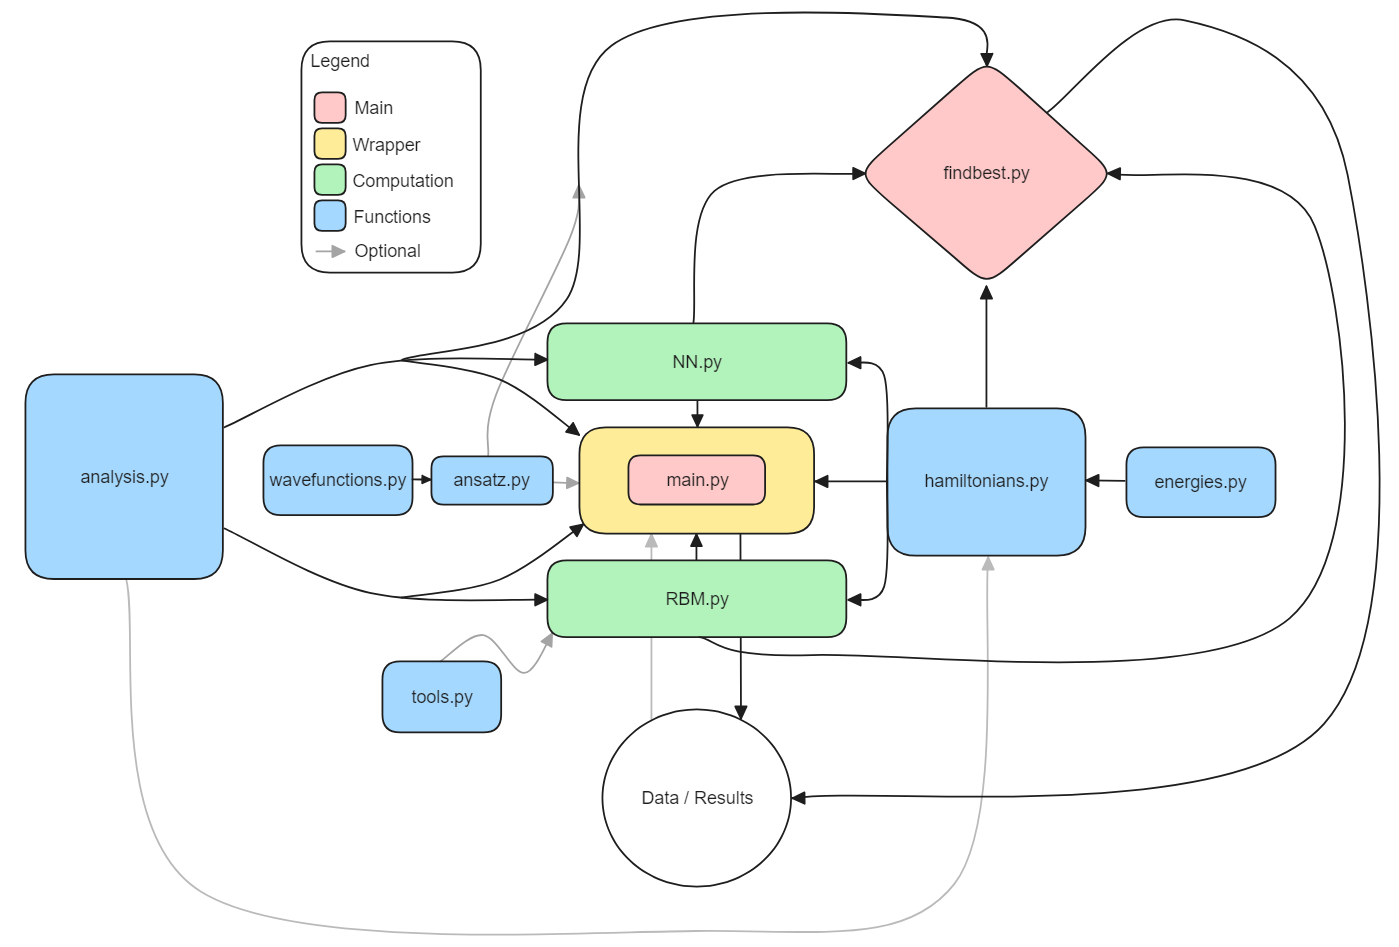
\includegraphics[scale=0.35]{codebasestructure.png}
    \caption{The structure of all code related to the project}
    \label{fig:code}
\end{figure}
\newline
Given that this is an object oriented approach to solving quantum mechanical systems there are (as you may see) a lot of dependencies across the different parts of the code base. \newline
We start in \texttt{main.py}, which is from where we call the functions. In \texttt{main.py}, we import from \texttt{hamiltonians.py} the hamiltonian we wish to use. These would then be passed as (for example, in the case of the harmonic oscillator) \texttt{NN('harmonic\textunderscore oscillator', args)} or \texttt{RBM('harmonic\textunderscore oscillator', args)} for the respective wrapper function called \texttt{run\textunderscore restricted\textunderscore boltzmann\textunderscore model()} or \newline  \texttt{run\textunderscore neural\textunderscore network\textunderscore model()} respectively. \newline
The wrapper functions take arguments in addition to the hamiltonian. In the case of the RBM, it takes the additional arguments: \texttt{num\textunderscore particles, num\textunderscore hidden, num\textunderscore samples, num\textunderscore iterations, runs, dof} and NN takes the same arguments, sans the \texttt{num\textunderscore hidden}. They also both have the optional boolean arguments, \texttt{verbose, load, debug}.
\newline
The wrapper \texttt{runner.py} then handles starting the computation of \texttt{NN.py} or \texttt{RBM.py}. If \texttt{runs > 1}, then it will calculate the mean and standard deviation of the results. \texttt{runner.py} can also optionally use \texttt{ansatz.py} to pre-train the network prior to computation. Here we use another trial wave function to get the initial weights of the neural network closer to the expected weights. If weights have already been generated, they are instead retrieved from the folder \texttt{/weights/}. These trial wave functions are stored in \texttt{wavefunctions.py} within the \texttt{Wavefunctions} object. \texttt{wavefunctions.py} also contains a seperate object called \texttt{Analytical}, which are the analytical solutions to the wave functions for the systems where it is applicable. This is mostly used for debugging. \newline
The implementation of \texttt{NN.py} and \texttt{RBM.py} we will discuss below in their respective implementation sections, but they have a few dependencies it would be better to discuss here:
\newline
Firstly, and perhaps the most obvious, is \texttt{hamiltonians.py}. \texttt{hamiltonians.py} is a collection of all compatible hamiltonians. Given that the NN and RBM models use different python libraries, the hamiltonian implementations are not shared between NN and RBM. There are respective \texttt{NN} and \texttt{RBM} objects which contain the hamiltonians implemented for each model architecture. Each method within the objects calculates $\hat H \psi(x)$ given $\psi$ and $x$ \newline 
Within each of these objects are implementations for the hamiltonians \newline \texttt{harmonic\textunderscore oscillator}, \texttt{two\textunderscore fermions}, \texttt{calogero\textunderscore sutherland}, \texttt{ising} and \texttt{heisenberg}. \newline \texttt{hamiltonians.py} also depends on \texttt{energies.py}, which contains an object \texttt{Energies} that contains the analytical ground state energy for each hamiltonian. If the ground state energy is not exactly known, we have used NetKet to approximate polynomials for the energy. \newline
Lastly we have the \texttt{analysis.py}, which simply contains helper functions that better let us interpret our results. Functions such as plotting the relative error, the particle density, the wave function or the particle density over all iterations.
\subsection{Training parameter optimization}
We also have one other section of the code, \texttt{findbest.py}, which aims to optimize the selection of the step size $\delta$ and learning rate $\eta$ by forming a forming a grid of them and looking at which combination gives the lowest relative error. Unlike \texttt{main.py} and \texttt{runner.py}, \texttt{findbest.py} has no wrapper and instead serves as a combination of \texttt{main.py} and \texttt{runner.py}. We can again optionally invoke the use of pre-training, if desired by using \texttt{ansatz.py}. Again, given that there are two different approaches and libraries in use, there are seperate functions \texttt{findbestNN()} and \texttt{findbestRBM()} They both take the same arguments as those in \texttt{main.py}, with the caveat that they can take lists of $\delta$ and $\eta$-values, lists of hamiltonians (as a list of strings) and, as computation time can be quite long, a boolean \texttt{sound} which controls whether or not a sound will be played when computation is finished. \newline
The results will then be saved to \texttt{findbestNN.txt} or \texttt{findbestRBM.txt} respectively.
\section{How to use} \label{howto}
Simply run either \texttt{run\textunderscore restricted\textunderscore boltzmann\textunderscore machine()} or \texttt{run\textunderscore neural\textunderscore network \textunderscore model()} with the appropriate parameters filled in. Here are some example runs:
\begin{lstlisting}[language=Python]
    #RBM, a single two fermions model run with 2 visible units, 8 hidden units, 
    # 500 samples over 250 iterations with 2 degrees of freedom
    run_restricted_boltzmann_model(RBM('two_fermions', 1), 2, 8, 500, 250, 1, 2)
\end{lstlisting}
\begin{lstlisting}[language=Python]
    #NN, three runs of the harmonic oscillator model run with 1 particle, 
    # 2000 samples over 1000 iterations with 1 degrees of freedom
    run_neural_network_model(NN('harmonic_oscillator', 1), 1, 2000, 1000, 3, 1)
\end{lstlisting}
\newpage
\section{Model architecture}
\subsection{Weight Initialization}
We've talked a lot about the weights themselves, but have neglected to mention how we're going to initialize them. There are many different ways to initialize them, and we don't strictly always need to, but it is a good idea to. After all, if all weights start with the same values, then all neurons will learn the same features, and the network will be unable to learn complex patterns. \newline
In the case of our RBM model, RBMs are commonly initialized by making $a$ and $b$ zero vectors of length $x$ and $h$ respectively. $W$ we initialize as a random as a normal distribution of size $(x, h)$, giving:
\begin{equation*}
    \Vec{a} = [0, 0, 0, ..., 0]
\end{equation*}
\begin{equation*}
    \Vec{b} = [0, 0, 0, ..., 0]
\end{equation*}
\begin{equation*}
    \Vec{W} = S \left[\begin{matrix}
        G_{1,1}& G_{2, 1}& \dots& G_{N,1}  \\
        G_{1,2}&  G_{2,2}& \dots& G_{N,2} \\
        \vdots& \vdots& \ddots& \vdots \\
        G_{1,M}& G_{2, M}& \dots& G_{N, M}
    \end{matrix}\right]
\end{equation*}
where S is a scaling factor, and $G$ is a normal distribution. In this work we set $S=0.01$. \newline
In the case of our Neural Network, we will use the Xavier normal distribution, also known as Glorot initialization \cite{glorot}, where we sample initial weights from the distribution:
\begin{equation*}
    w_i = G(0, \text{std}^2)
\end{equation*}
where $G$ is the normal distribution and std is the standard deviation given as:
\begin{equation*}
    \text{std} = \text{gain} \times \sqrt{\frac{2}{\text{fan\textunderscore in} + \text{fan\textunderscore out}}}
\end{equation*}
where gain is a scaling factor applied to the standard deviation, and fan\textunderscore in is the number of inputs in a layer, fan\textunderscore out is the number of outputs of a layer. For ReLU activation functions, it is recommended to set gain to $\sqrt{2}$.
\newpage
\subsection{Choice of network sizes}
As our code is intended as a one-size-fits-all Neural Network, we'll be using the same network size across all our systems. For our RBM model, we have chosen a total of $4$ hidden units for all systems. The choice of the number of hidden units is a case of trial and error, as there is no exact recipe for deciding how many hidden units are best. It's is a case of a three-piece venn-diagram between run times, model complexity and system complexity. We need to find the perfect $h$ where it is the best for all the systems on average, where we don't compromise too much on the model-complexity, but also not make the model either overly complex (there is such a thing as too complex of a model).\newline
For the FFNN model, we have decided on a three hidden layers 'funnel' shaped system, of dimensions $64:32\times32:1$. Our input layer is $M:64$, where $M$ is \texttt{num\textunderscore particles}$\times$ $\texttt{dof}$. This leads to generally stable training whilst also yielding relatively good results for most systems. After each of our hidden layers we employ the ReLU activation function. We use no activation function on our output.
\subsection{Choice of system parameters}
Choice of system parameters is a balancing act. As we increase the number of samples, so too must we increase the number of iterations, provided we do not already have a good ansatz for the probability distribution of $|\Psi(x)|^2$. For example, in the case of the 1D Harmonic Oscillator, we know that it is Gaussian, so we do not need many iterations for our Metropolis-Hastings algorithm to generate a good set of samples for the distribution. We can also implement early stopping to neglect entirely the choice of iterations. \newline
Another parameter we have to choose (for relevant systems, atleast), is the number of particles. Generally, as the number of particles increase, so too does the numerical complexity. In turn, it will likely be harder for our systems to approximate the ground state for higher dimension systems (here dimension means $M$, that is \texttt{num\textunderscore particles}$\times$ $\texttt{dof}$). Therefore we must expect an increase in iterations as we increase the system complexity, and we must also expect to increase the number of samples so as to get a sufficient distribution for the given system.
\newpage
\subsection{Choice of learning and step parameters}
Lastly we have the choice of our learning parameters. These are $\eta$, which is the rate at which the network learns as discussed in Sec. [\ref{opt}], and $\delta$, which is the step-length taken by the Metropolis-Hastings algorithm, as mentioned in Sec. [\ref{metro}]. The higher $\eta$, the higher the chance that we overshoot or 'over-fit' our results. The higher $\delta$, the lower the acceptance ratio of the sampling method will be as we run a bigger risk of stepping outside of the distribution. It $\eta$ is too low, then convergence will take too long or we will get stuck in local minima. If $\delta$ is too low, then the sampling will do very little to get us to the correct distribution (provided we are not already there). \newline
As these parameters are so specific to each problem, we will use different parameters $\eta$ and $\delta$ for each system, and we will use a grid-search to find the combination (for lattice systems, this is only a search across $\eta$ as $\delta$ goes unused).
\section{Libraries}
\subsection{PyTorch} \label{PyTorch}
For our neural network we'll be using the PyTorch library. PyTorch will serve as both the means to represent the wave function (that is the neural network) and also handle the gradient calculation. There are several gradient calculations to be done. For the Hamiltonians, we see that they feature the Laplacian (double derivative). As such, we can use PyTorchs \texttt{autograd()} method. We can calculate the derivative of some function $f(x) = x^3$, let us say we want to evaluate both $\frac{d}{dx} f(x)$ and $\frac{d^2}{dx^2} f(x)$ at $x=2$. This is trivial to do by hand:
\begin{equation*}
    \frac{d}{dx} f(x) = 3x^2 \xrightarrow[]{} f'(2) = 12
\end{equation*}
\begin{equation*}
    \frac{d^2}{dx^2} f(x) = 6x \xrightarrow[]{} f''(2) = 12
\end{equation*}
\newpage
Let us now do this again, this time in PyTorch:
\begin{lstlisting}[language=Python]
    import torch

    x = torch.tensor(2., requires_grad=True)
    y = x**3
    
    first = torch.autograd.grad(y, x, create_graph=True)[0]
    second = torch.autograd.grad(first, x)[0]
    
    print(f'First derivative of f({x}):', first.item())
    print(f'Second derivative of f({x}):', second.item())

    # First derivative of f(2.0): 12.0
    # Second derivative of f(2.0): 12.0
\end{lstlisting}
Let us now up the difficulty, consider the function
\begin{equation*}
    f(x, y) = 5x^4 - 5yx^2 + 3y^3 - 55y + xy - 3
\end{equation*}
Let us evaluate it at the point $(3, 3)$, and we find:
\begin{equation*}
    \frac{\partial}{\partial x} f(x, y) = 20x^3 - 10xy + y
\end{equation*}
\begin{equation*}
    \frac{\partial^2}{\partial x^2} f(x, y) = 60x^2 - 10y 
\end{equation*}
\begin{equation*}
    \frac{\partial}{\partial y} f(x, y) = -5x^2 + x + 9y^2 - 55
\end{equation*}
\begin{equation*}
    \frac{\partial^2}{\partial y^2} f(x, y) = 18y
\end{equation*}
Thus giving:
\begin{equation*}
    \nabla f(3, 3) = (453, -16)
\end{equation*}
\begin{equation*}
    \nabla^2 f(3, 3) = (510, 54)
\end{equation*}
\newpage
and the accompanying code:
\begin{lstlisting}[language=Python]
    func = 5*x**4 - 5*y*x**2 + 3*y**3 - 55*y + x*y - 3

    first_x = torch.autograd.grad(func, x, create_graph=True)[0]
    first_y = torch.autograd.grad(func, y, create_graph=True)[0]

    second_x = torch.autograd.grad(first_x, x)[0]
    second_y = torch.autograd.grad(first_y, y)[0]

    print(f'First derivative of f({x}, {y}):', (first_x.item(), first_y.item()))
    print(f'Second derivative of f({x}, {y}):', (second_x.item(), second_y.item()))

    # First derivative of f(3.0, 3.0): 453.0, -16.0
    # Second derivative of f(3.0, 3.0): 510.0, 54.0
\end{lstlisting}
Now of course, the systems in question are much more complex than these. Typically a neural network will have thousands of trainable parameters, and while these parameters aren't important when we're evaluating $\Psi$ with respect to coordinates like $x, y$, they are important when we're updating the neural network
\newline
And therein lies the other use of gradient calculation we'll be using with PyTorch, the training of the network itself.
\newpage
For PyTorch, this is handled in the backward() method. Consider this relatively simple model:
\begin{lstlisting}[language=Python]
import torch
import torch.nn as nn
class NeuralNetwork(nn.Module):
    def __init__(self, N):
        super(NeuralNetwork, self).__init__()
        self.N = N
        self.model = nn.Sequential(
            nn.Linear(self.N, 25),
            nn.ReLU(),
            nn.Linear(25, self.N),
        )
 
    def forward(self, x):
        return self.model(x)
    
def targetfunc(x):
    return x**3 - 5*x + 3 

N = 50

x = torch.linspace(-5, 5, N)

y_values = targetfunc(x)

NN = NeuralNetwork(N)
MSE = nn.MSELoss()

optimizer = torch.optim.Adam(NN.model.parameters())

pytorch_total_params = sum(p.numel() for p in NN.model.parameters() if p.requires_grad)
print('Total trainable parameters:', pytorch_total_params)

for epoch in range(500):
    optimizer.zero_grad()
    y_pred = NN(x)
    loss = MSE(y_values, y_pred)
    loss.backward()
    optimizer.step()
    if epoch % 10 == 0:
        print(loss.item())
\end{lstlisting}

This model yields $2575$ (!!) trainable parameters, for all of which we must evaluate $\frac{\partial}{\partial w_i}\text{NN}(x)$, where $w_i$ is a given weight. Luckily the \texttt{backward()} does this very quickly.
\subsection{JAX} \label{Jax}
For the JAX implementation, it serves much the same purpose as that of the PyTorch implementation, that is calculating the gradients. Consider the sample example as before, we wish to calculate the first and second derivative of $f(x) = x^3$:
\begin{lstlisting}[language=Python]
    import jax

    x = 2.
    y = lambda z : z**3
    
    grad = jax.grad(y)
    grad2 = jax.grad(grad)
    
    first = grad(x)
    second= grad2(x)
    
    print(f'First derivative of f({x}):', first)
    print(f'Second derivative of f({x}):', second)
    # First derivative of f(2.0): 12.0
    # Second derivative of f(2.0): 12.0
\end{lstlisting}
Similarly, we get:
\begin{lstlisting}[language=Python]
    x = 3.
    y = 3.
    
    def fun(x, y):
        return 5*x**4 - 5*y*x**2 + 3*y**3 - 55*y + x*y - 3
    
    grad = jax.grad(fun, argnums=(0, 1))
    
    grad2 = jax.jacobian(grad, argnums=[0, 1])
    
    first = grad(x, y)
    second = grad2(x, y)
    
    second_x = second[0][0]
    second_y = second[1][1]
    
    print(f'First derivative of f({x}, {y}):', first[0], first[1])
    print(f'Second derivative of f({x}, {y}):', second_x, second_y)
    # First derivative of f(3.0, 3.0): 453.0 -16.0
    # Second derivative of f(3.0, 3.0): 510.0 54.0
\end{lstlisting}
Note the use of the Jacobian to calculate the second derivative. This is the result of a quirk with JAX where it will not calculate the second gradient with respect to two arguments, so we must use this workaround.
\newline
Now we move on to the other gradient calculation, unlike the neural network which can have any number of weights, the RBM has the visible weights $a_i$, the hidden weights $b_j$ and the weights between them $w_{ij}$, where their respective sizes are dependent on the number of visible and hidden units.
\newline
We calculate then the loss function explicitly using $W, a, b$, and then use these as the \texttt{argnums} for the gradient calculation. This tells JAX that it should differentiate with respect to these parameters, from which we get their gradients, which we can then use to minimize the loss, as so:
\begin{lstlisting}[language=Python]
import jax

grad = jax.value_and_grads(fun, argnums=(0, 1, 2))
loss, grads = grad(W, a, b, x)
update_gradients(grads)

\end{lstlisting}
\subsection{NetKet}
While not strictly part of our computational pipeline, we have used the NetKet library with basis in \cite{nkheisenberg} as this system doesn't have an exact solution. We have therefore solved the Heisenberg system for several different particle numbers to approximate a polynomial as a solution to this system specifically. This solution is approximated as:
\begin{equation*}
    E_0 \approx -(- 0.0007 L^3 + 0.02905L^2 - 2.1175L + 0.7008)
\end{equation*}
which was obtained by fitting a cubic function to the results by using NetKet for $2N$ particles with $N$ $\in (1, 12)$
\newpage
\section{Computational pipeline}
Let us now go through the computational pipeline. Note that the code is somewhat simplified and should be treated more as pseudo-code than the real thing \newline
We start of course within the variational monte carlo itself, as:
\begin{lstlisting}[language=Python]
def variational_monte_carlo(psi, hamiltonian, num_particles, num_samples
                            num_iterations, learning_rate, dof, delta):

    if hamiltonian.spin:
        samples = [where(random(num_samples, dof) > 0.5, 0.5, -0.5) for _ in range(num_particles)]
    else:
        samples = [random(num_samples, dof) for _ in range(num_particles]

    samples = concat(samples, dim-1)


    for iterations in range(num_iterations):

        psi_norm = normalize(psi, samples, hamiltonian.name)

        if hamiltonian.spin:
            samples = metropolis_hastings_update(samples, num_particles, psi_norm, delta, hamiltonian.name)
        else:
            samples = metropolis_hastings_spin_update(samples, psi_norm)

        psi_norm = normalize(psi, samples, hamiltonian.name)


        loss_value = loss(psi, hamiltonian, samples)

        update_weights(loss_value)

        psi_norm = normalize(psi, samples, hamiltonian.name)


    return loss_value
    
\end{lstlisting}
\newpage
Our samples pass through a few different functions, let's start from the top:
\begin{lstlisting}[language=Python]
def normalize(psi, samples, name):

    psi_vals = psi(samples)
    psi_magnitude_squared = square(psi_vals)
    integral = sum(psi_magnitude_squared)

    def normalized(x):
        return psi(x) / sqrt(integral)

    return normalized
\end{lstlisting}
For free moving particles
\begin{lstlisting}[language=Python]
def metropolis_hastings_update(x, num_particles, psi, delta, hamiltonian.name):
    
    F = quantum_force(x, psi)
    idx = randint()

    new_x[idx] = x[idx] + sqrt(delta) * random() + 0.5*delta*F[idx]

    psi_x = psi(x)
    new_psi_x = psi(new_x)

    G = greensfunction(x, new_x, F, delta)

    A = min(1, G*(new_psi_x**2/psi_x**2))

    rnd_numbers = random()

    acceptance_mask = rnd_numbers < A

    x = where(acceptance_mask, new_x, x)

    return x
\end{lstlisting}
where:
\begin{lstlisting}[language=Python]
def quantum_force(x, psi):
    psi_x = psi(x)
    grad_psi = gradient(psi_x, x)
    force = 2*grad_psi/psi_x
    return force
\end{lstlisting}
\newpage
and:
\begin{lstlisting}[language=Python]
def greensfunction(x, new_x, F, delta, dof):
    num_samples, dof = x.shape
    N = dof  
    D = 0.5
    
    normalization_factor = 1 / (4 * torch.pi * D * delta)**(0.5 * N)
    
    diff = proposed_x - x - D * delta * F
    exponent = -torch.sum(diff**2, dim=1) / (4 * D * delta)
    
    G = normalization_factor * torch.exp(exponent)
    return G
\end{lstlisting}
For lattice particles:
\begin{lstlisting}[language=Python]
def metropolis_hastings_spin_update(samples, psi):
    M, N = samples.shape

    idx = randint()

    new_samples = samples.clone()
    new_samples[idx] *= -1

    psi = psi(samples)
    new_psi = psi(new_samples)

    A = min(1, (new_psi_x**2/psi_x**2))

    rnd_numbers = random()

    acceptance_mask = rnd_numbers < acceptance_prob

    samples = where(acceptance_mask, new_samples, samples)

    return samples
\end{lstlisting}
Lastly we have the loss function:
\begin{lstlisting}[language=Python]
def loss(psi, hamiltonian, samples):
    H_psi = hamiltonian.hamiltonian(psi, samples)

    psi_vals = psi(samples)

    local_energy = H_psi / psi_vals
    local_energy = mean(local_energy)

    return local_energy
\end{lstlisting}
Note that these codes will not be 1:1. There are small differences between the implementations of the RBM and NN respectively, so this serves as a compromise between the two to give a general idea as to what we've produced. For a more rigorous look, you may refer to the github repository linked in the introduction Sec. [\ref{git}].
\section{The 1D Harmonic Oscillator}
The hamiltonian for the 1D Harmonic Oscillator is implemented as:
\begin{lstlisting}[language=Python]
def harmonic_oscillator(psi, x)
    psi_x = psi(x)
    gradient_psi_x = gradient(psi_x, x)
    gradient_psi_x2 = gradient(gradient_psi_x, x)

    kinetic_energy = - 1/2 * gradient_psi_x2
    potential_energy = 1/2 * omega**2 * x**2 * psi_x

    H_psi = kinetic_energy + potential_energy

    return H_psi
\end{lstlisting}
This is a rather trivial hamiltonian and should be self-explanatory.
\section{The Two Fermions Model}
The hamiltonian for the Two Fermions model is implemented as:
\begin{lstlisting}[language=Python]
def two_fermions(psi, x)
    psi_x = psi(x)
    gradient_psi_x = gradient(psi_x, x)
    gradient_psi_x2 = gradient(gradient_psi_x, x)

    kinetic_energy = - 1/2 * gradient_psi_x2
    potential_energy = 1/2 * omega**2 * x**2 * psi_x

    r1 = x[:, :2]
    r2 = x[:, 2:]

    r12 = norm(r1 - r2)

    interaction_energy = (1 / r12)*psi_x

    H_psi = kinetic_energy + potential_energy + interaction_energy

    return H_psi
\end{lstlisting}
Again, this Hamiltonian is trivial and needs no explanation
\section{The Calogero-Sutherland Model}
\begin{lstlisting}[language=Python]
def calogero_sutherland(psi, x):

        N, M = x.shape
        psi_x = psi(x) 
        gradient_psi_x = torch.autograd.grad(psi_x, x, grad_outputs=torch.ones_like(psi_x), create_graph=True)[0]
        
        laplacian_psi_x = torch.autograd.grad(gradient_psi_x, x, grad_outputs=torch.ones_like(gradient_psi_x), create_graph=True)[0]
        
        
        kinetic_energy = -0.5 * laplacian_psi_x

        r_squared = x**2
        potential_energy = 0.5 * omega**2 * r_squared*psi_x
        
        interaction_energy = 0
        for i in range(M):
            for j in range(i + 1, M):
                x_ij = positions[:, i] - positions[:, j]
                interaction_energy += beta * (beta - 1) * (torch.tanh(x_ij / x_0)**2) / (x_ij**2)
        
        H_Psi = kinetic_energy.sum(axis=1) + potential_energy.sum(axis=1) + interaction_energy * psi_x


        return H_Psi
\end{lstlisting}
Here, we have much the same model as above except the interaction term is instead replaced with a scaling interaction term. We start with a low scale such that the system can hopefully get a good estimation of the wave function before we slowly introduce a strong and stronger interaction until we get close enough that we have a good estimate of the ground state energy.
\section{The 1D Transverse Field Ising Model}
The Ising model is implemented as:
\begin{lstlisting}[language=Python]
def ising(psi, spins):

    N, M = spins.shape
    
    interaction_term = zeros(N)
    for i in range(M):
        interaction_term -= V * spins[:, i] * spins[:, (i+1) % M] * psi(spins)
    
    transverse_term = zeros(N)
    for i in range(M):
        flipped_spins = spins.clone()
        flipped_spins[:, i] *= -1
        transverse_term -= Gamma * psi(flipped_spins)
    
    H_Psi = interaction_term + transverse_term

    return H_Psi
\end{lstlisting}
We calculate first the interaction term between spin $i$ and spin $i+1$. We assume periodic boundary conditions. After that, we flip spins so as to calculate the transverse term.
\section{The 1D Heisenberg Model}
The Heisenberg model is implemented as:
\begin{lstlisting}[language=Python]
def heisenberg(psi, spins):
    N, M = spins.shape
    H_Psi = zeros(N)
    
    for i in range(M):
        next_i = (i + 1) % M
        
        flipped_spins_xx = spins.clone()
        flipped_spins_xx[:, i] *= -1
        flipped_spins_xx[:, next_i] *= -1
        
        flipped_spins_yy = spins.clone()
        flipped_spins_yy[:, i] *= -1
        flipped_spins_yy[:, next_i] *= -1
        
        sigma_z_term = spins[:, i] * spins[:, next_i]
        
        H_Psi += J * (psi(flipped_spins_xx) + psi(flipped_spins_yy) + sigma_z_term * psi(spins))

    
    return H_Psi
\end{lstlisting}
Here we iterate through each particle $i$ and flip the spins of it and its next door neighbour $i+1$. We again assume periodic boundary conditions.
\newpage
~\newpage
\part{Results}
\section{Hamiltonians}
\subsection{The 1D Harmonic Oscillator}
\subsubsection*{Neural Network}
We start by estimating the ground state energy of the system over an average of 10 runs giving us:
\begin{figure}[ht!]
    \centering
    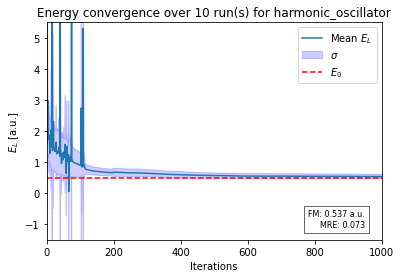
\includegraphics[scale=0.65]{NN_harmonic10.png}
    \caption{The energy convergence of our FFNN model of a 1D Harmonic Oscillator system. Deviates by 7\% for $\eta = 1 \times 10^{-3}, \; \delta = 1 \times 10^{-3}$.}
    \label{fig:NNho}
\end{figure}\newline
This yields relatively good results, and serves as a good benchmark for our Network model. As expected, the variance is reduced as the training converges, and we approach a good estimation of the ground state energy, landing at a deviation of $7\%$ after 1000 iterations. This was done for the best found $\eta$ and $\delta$.
\newpage
\subsubsection*{Restricted Boltzmann Machine}
Let us now move on to the benchmarking of the RBM model.
\begin{figure}[ht!]
    \centering
    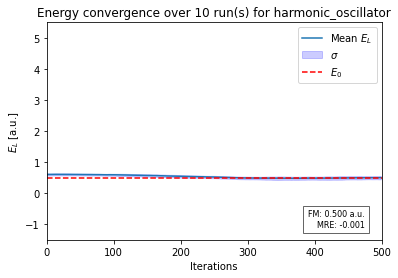
\includegraphics[scale=0.65]{RBM_harmonic10.png}
    \caption{The energy convergence of our RBM model of a 1D Harmonic Oscillator system. Deviates by .1\% for $\eta = 1 \times 10^{-3}, \; \delta = 5 \times 10^{-2}$.}
    \label{fig:RBMho}
\end{figure}
\newline
For the RBM model, we see that it performs even better than that of the Neural Network model, as it is almost a perfect. This is a a very promising result. Additionally, the RBM models seems to be much more stable and experiences much less variance than that of the NN model.
\newpage
\subsection{The Two Fermions Model}
We now move on to a two-dimensional model, that of the Two-Fermions model.
\subsubsection*{Neural Network}
\begin{figure}[ht!]
    \centering
    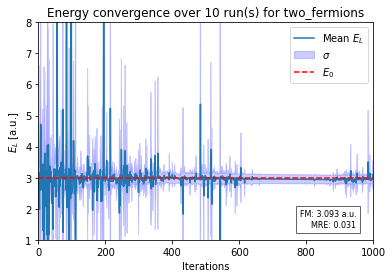
\includegraphics[scale=0.65]{NN_twofermions10.png}
    \caption{The energy convergence of our FFNN model of a 2D Two Fermions system. Deviates by 3\% for $\eta = 1 \times 10^{-3}, \; \delta = 1 \times 10^{-3}$.}
    \label{fig:NNtf}
\end{figure}
We see now significantly more noise than that of the first model. As we near the end, the variance decreases but there is still some noise even at the very end. Still, even with the noise we only see a $3\%$ deviation from the known ground state energy, giving more confidence that our model is robust
\newpage
\subsubsection*{Restricted Boltzmann Machine}
\begin{figure}[ht!]
    \centering
    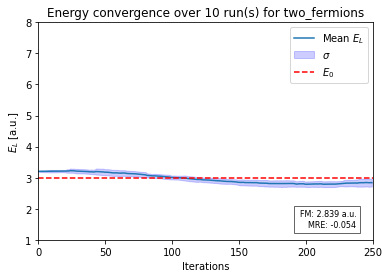
\includegraphics[scale=0.65]{RBM_twofermions10.png}
    \caption{The energy convergence of our RBM model of a 2D Two Fermions system. Deviates by 5\% for $\eta = 1 \times 10^{-3}, \; \delta = 5 \times 10^{-2}$.}
    \label{fig:RBMtf}
\end{figure}
For the RBM variant, we see much the same results as we saw with the 1D Harmonic Oscillator: Slow convergence and little noise. We see a $5\%$ deviation which is still good, but we also see that the energy goes below $E_0$
\newpage
\subsection{The 1D Transverse Field Ising Model}
Now for the lattice systems:
\subsubsection*{Neural Network}
\begin{figure}[ht!]
    \centering
    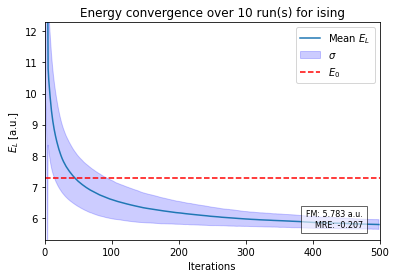
\includegraphics[scale=0.65]{NN_ising10.png}
    \caption{The energy convergence of our FFNN model of a 1D Transverse-Field Ising system. Deviates by 21\% for $\eta = 1 \times 10^{-3}$ for 6 particles}
    \label{fig:NNtfi}
\end{figure}
Here we run into our first blunder. The Ising model converges well below that of the expected ground state energy, with a deviation of $21\%$. This is unexpected, but is explored in App. [\ref{appendixb}]
\newpage
\subsubsection*{Restricted Boltzmann Machine}
\begin{figure}[ht!]
    \centering
    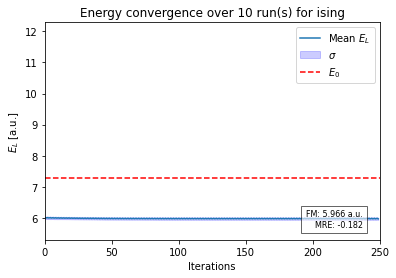
\includegraphics[scale=0.65]{RBM_ising10.png}
    \caption{The energy convergence of our RBM model of a 1D Transverse-Field Ising system. Deviates by 18\% for $\eta = 5 \times 10^{-2}$ for 6 particles}
    \label{fig:RBMtfi}
\end{figure}
Again, we see the energy converge to a value below that of the expected value, deviating with $18\%$. While this is bad, it is also reassuring because both models converge to approximately the same value, indicating the error lies in our specific Ising implementation, not the models themselves. More on this in App. [\ref{appendixb}]
\newpage
\subsection{The 1D Heisenberg Model}
\subsubsection*{Neural Network}
\begin{figure}[ht!]
    \centering
    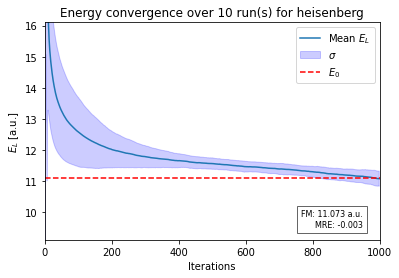
\includegraphics[scale=0.65]{NN_heisenberg10.png}
    \caption{The energy convergence of our FFNN model of a 1D Heisenberg system. Deviates by .3\% for $\eta = 1 \times 10^{-4}$ for 6 particles}
    \label{fig:NNhb}
\end{figure}
Here we see again a good convergence to the expected value of $E_0$. It is worth noting that, as mentioned, the $E_0$ for the Heisenberg system is a cubic fit of the NetKet solutions. The deviation is only $.3\%$, one of our best results yet, but the convergence isn't entirely flat and there is a fair bit of variance even as we reach the supposed convergence point.
\newpage
\subsubsection*{Restricted Boltzmann Machine}
\begin{figure}[ht!]
    \centering
    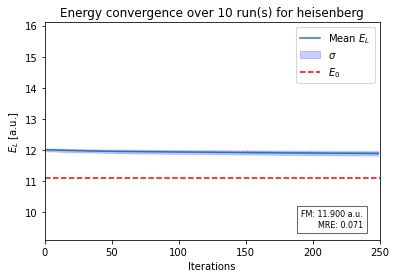
\includegraphics[scale=0.65]{RBM_heisenberg10.png}
    \caption{The energy convergence of our RBM model of a 1D Heisenberg system. Deviates by 7\% for $\eta = 1 \times 10^{-3}$.}
    \label{fig:RBMhb}
\end{figure}
For the RBM model, we see much the same behavior as we saw with its Ising model. An entirely flat energy almost devoid of learning. This is indicative of our model not necessarily working well with lattice systems, but it is still a deviation of only $7\%$, which is not the worst.
\newpage
\subsection{The Calogero-Sutherland Model}
\subsubsection*{Neural Network}
\begin{figure}[ht!]
    \centering
    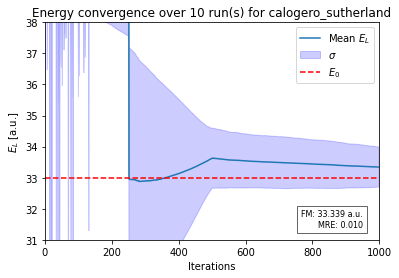
\includegraphics[scale=0.65]{NN_cs10.png}
    \caption{The energy convergence of our FFNN model of a 1D Calogero-Sutherland system. Deviates by 1\% for $\eta = 1 \times 10^{-3}, \; \delta = 1 \times 10^{-3}$ for 6 particles}
    \label{fig:NNcs}
\end{figure}
We now move on to the most difficult system we're going to be studying. As mentioned when presenting this system, we need to approximate the interaction between the particles. Ideally, the model can then learn the system for little to no interaction, and as we slowly turn on the interaction we see the model approach $E_0$ as $x_0$ approaches $0$. As a compromise to this, we let $x_0$ go from $1$ to $0.68$, which yielded the results above, a deviation of just $1\%$.
\newpage
\subsubsection*{Restricted Boltzmann Machine}
\begin{figure}[ht!]
    \centering
    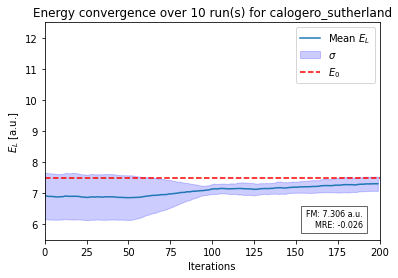
\includegraphics[scale=0.65]{RBM_cs10.png}
    \caption{The energy convergence of our RBM model of a 1D Calogero-Sutherland system. Deviates by 2\% for $\eta = 1 \times 10^{-3}, \; \delta = 5 \times 10^{-2}$ for 3 particles}
    \label{fig:RBMcs}
\end{figure}
Lastly we look at the RBM version. Again, we let $x_0$ go from $1$ to $0.68$, but this time for fewer particles, showing that it is still a good compromise for different numbers $N$. We see a deviation of only $2\%$.
\newpage
~\newpage
\part{Discussion}
\section{Results discussion}
Generally, the results are a mixed bag. For some systems, our models work great, and for others, the results are mediocre. All the results have at least some merit, there are no outright awful results, and we have at least shown that our model is capable of approximating the wave function of some Hamiltonians very well while approximating others with a degree of uncertainty. We do see most models converge close to the analytical solution, but in some cases, it appears as if it still hasn't reached a true convergence. Some cases, none of which were included in the selected results above, don't seem to converge at all. This was dependent on both the network structure and the system chosen to study and its parameters. Still, it has to be said that there are definitely some improvements to be made. Some examples of these improvements could be performance improvements for the RBM model or different energy models to choose from, or in the case of the FFNN implementation, a more robust network that is not so prone to \texttt{NaN}s and \texttt{inf}s (more on that later), such that we can have a deeper network that can more intricately approximate and learn the wave function of a given Hamiltonian.
\newpage
\subsection{Further discussions on $x_0$}
While the original paper \cite{jane} from which we got the idea of the scaling $x_0$ parameter let $x_0$ go all the way to zero, we were not able to do this and still get reasonable results. As such, we had to make a compromise. We will now give some justification that this choice of not letting $x_0$ go all the way to $0$ still gets us an okay approximate. To prove this, we solve now the same system for 8, 10, 15 and 20 particles respectively and compare the solutions to the analytical solution:
\begin{figure}[ht!]
    \centering
    \subfigure(a){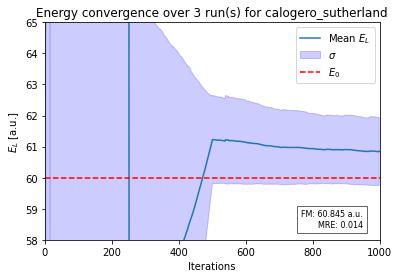
\includegraphics[width=0.45\textwidth]{611a.png}} 
    \subfigure(b){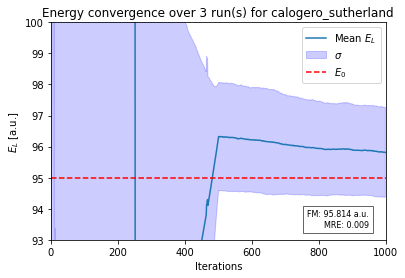
\includegraphics[width=0.45\textwidth]{611b.png}}
    \newline
    \centering
    \subfigure(c){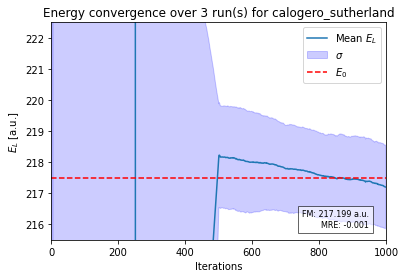
\includegraphics[width=0.45\textwidth]{611c.png}}
    \subfigure(d){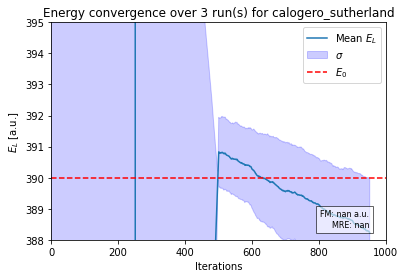
\includegraphics[width=0.45\textwidth]{611d.png}}
    \caption{For $N_{(a)} = 8$, $N_{(b)} = 10$, $N_{(c)} = 15$ and $N_{(d)} = 20$, respectively.
    \newline We see here how we get a relatively small error for this approximation \newline
    Note that we sadly got some \texttt{NaN}s for the final 50 iterations of the 20 particle case.}
    \label{fig:611}
\end{figure}
\newline
Now of course, this doesn't solve the actual problem, that our network (or we) are unable to properly learn the wave function of this system, however, it serves as a compromise that allows us to get some results. We also notice that for higher $N$, this approximation no longer holds up as well, as we are no longer seeing any convergence.
\section{Neural Network Architecture choice}
Another natural question to this is, which method do we prefer for solving neural networks between the Feed-Forward Neural Network and the Restricted Boltzmann Machine. Out of the box, FFNN was definitely easier to work with. This is natural, of course, as it requires little to no rigorous implementation of the wave function. One simply defines a network size and shape and goes. In contrast, the RBM model is a bit more restrictive to work with. Instead of picking just making the model and starting, we instead need to find out what kind of energy function we want to use (ie. do we want a Gaussian-Binary or a Binary-Binary RBM?), and then make sure that those energy models are compatible with all (relevant) inputs. That is not to say that the RBM is without merit. After all, unlike the FFNN, the RBM is inherently probabilistic in its definition. For the RBM, we can thus be sure that the wave function we have (from the beginning) is at least somewhat akin to a wave function. This might also explain why the RBM model initially started much lower than that of the FFNN model, which took time to converge at $E_0$, presumably because it still had to learn that it needs to 'be' probability amplitudes. \newline
In regards to performance, the FFNN model was significantly faster than that of the RBM model. This could be down to experience and knowledge, as we were entirely inexperienced with JAX, whereas we had some knowledge of Tensorflow (which could then be transferred onto PyTorch) prior to this project.
\section{Model complexity and stability}
One of the most important and interesting things to discuss is the impact of the model complexity. Looking at for example \cite{symm}, we see how even just small changes to the network architecture can have a significant impact on the complexity of the model, or rather how well it can portray/approximate the wave function. \newline Thus, since we wanted our model to be one-size-fits-all, we had to select a model that not only could portray all systems within a degree of error, but was also stable for all configurations. It is worth mentioned that this was not so much a problem with the RBM model as it was with the FFNN model. \newline
In regards to stability, a lot can go wrong when working with deep networks. We run the risk of over and underflows, causing seemingly random \texttt{NaN}s and \texttt{inf}s, so it is important that we take this in mind when choosing parameters for our network. In this regard, we found that the model was much stable when the initial (that is, the first hidden layer) was wide, hence the large first layer and subsequent funnel form of the net. For flat or 'bell-curve' (ie. where the the middle layers are bigger than the previous and the next, forming a pseudo bell curve over the network) nets, we found that the network was much less stable. It was therefore that we decided to go for a funnel shaped network with a wide initial net.
\newline
Interestingly, the two-fermions model was by far the most unstable. This perhaps makes sense when we study it's energy convergence Fig. [\ref{fig:NNtf}], as it was by far the most noisy of our systems. To us, this is indicative of a problem with higher degrees of freedom, as it was the only system where the degrees of freedom were not $1$. This also sadly meant that we were not able to use deeper networks, which might explain how the network was unable to approximate a wave function for some systems.
\section{Further improvements}
Perhaps one of the most glaring issues with the code as is is it's rigidity in terms of the Hamiltonians. Particularly, systems like Two-Fermions or the Harmonic Oscillator are (somewhat arbitrarily) restricted to 2 and 1 degree of freedom, meaning that the system has less flexibility than intended. \newline
Perhaps the best remedy to this would simply be to combine these two models into one. After all, they are quite similar, the only real difference being the interaction term and the move into 2 dimensions. The Two fermions model can also easily be extended to three dimensions without any additional adjustments. This leaves us only with the issue of particles, which we can fix simply by updating the interaction calculation to account for all particles, as opposed to calculating the interaction between just two. 
\newline
Another interesting feature to add would be that of a modular potential. That is, add a new object \texttt{potentials}, within which we can store the existing potentials. This gives us more flexibility in the systems we wish to study, letting us either use the existing potential, or define our own by passing, for example, a \texttt{lambda} statement as the potential, which in theory should work fine for any potential where it's decided by the distance to the origin. For other types of potentials, a bit more tweaking may be required, but we believe this is still a realistic addition to be made.
\newline
Adjacent to adding different potentials would also be adding different methods. For example, new or different sampling methods that allow for more 'views' with which to study the Hamiltonians.
\section{Criticism: The scope of the thesis}
With all of the discussion above, we believe therefore that we may have stretched ourselves a bit too thin with this thesis. Perhaps we would've been better served with focusing on either just neural networks or just the RBM, maybe using the other as just a benchmark for only a few systems and then really focusing on pushing the remainder to its limits (within reason). We could for example have used existing results from previous theses that used RBMs \cite{flugsrud} \cite{nordhagen}, and compared those results to the FFNN results of our own. \newline
Another idea would've been to instead consider fewer but more similar Hamiltonians and employ the modular potential suggestions from above to study them. This would've in turn (presumably) allowed us to study more variants of a single Hamiltonian with less of the headache of implementing an entirely new Hamiltonian (and everything that brings). It would've also presumably made for some interesting results.
\newpage
~\newpage
\part{Conclusion}
In summary, we've embarked on developing a series of software tools aimed at studying different Hamiltonian systems through the lens of the Variational Monte Carlo method. We began by first comprehensively exploring the Variational Monte Carlo, delving into it's mathematical basis and background before we layer by layer constructed a basis from which we could launch our numerical investigation.
\newline
Subsequently, we implemented respectively two distinct models, that of JAX-utilizing Restricted Boltzmann Machine and a PyTorch-utilizing Feed-Forward Neural Network. We find that these are network architectures are adept at accurately modeling some systems, this adeptness holding a particular promise as it addresses one of the main weaknesses of the traditional Variational Monte Carlo, the selection of a fitting ansatz, which this method solves .
\newline
We anticipate therefore that such approaches will significantly broaden the accesibility and utility of Variational Monte Carlo methods with respect to Quantum Mechanics. Moreover, it underscores the transformative potential of leveraging neural networks to refine and/or expedite computational methods, not just within quantum mechanics but within all of science. By harnessing these technologies, we aim not only to advance our understanding of complex physical systems, but to also pave the wave for more efficient and scalable computational methodologies in quantum mechanics and beyond \newline
This work was based not only on the origins of the Neural Quantum State \cite{NQS}, but also the work of previous graduates Flugsrud \cite{flugsrud} and Nordhagen \cite{nordhagen}, whom both undertook a similar endavour before us. We hope therefore that this addition to this library of studies into solving quantum mechanical systems using a neural networks will prove to be not only useful but also easy to employ for both future graduates but also for science as a whole.
\newpage
\section{Future work}
For future work or further iterating on the software we've developed, we've selected a few
\begin{itemize}
    \item Studying a or several Hamiltonian for different potentials, with a modular and objective oriented approach for easy use.
    \item Introduce different RBM energy models. There are many different energy models that are not even discussed here, and they could perhaps lend themselves very well to certain systems. This in turn means that we can achieve an even greater degree of customizability and learnability for the RBM model by introducing more energy models that are better suited for particular physical systems.
    \item Further improvements into deep learning and the correlation between network size/shape and its adaptability/correlation to a particular system
\end{itemize}
\newpage
~\newpage
\bibliographystyle{unsrtnat}
\bibliography{citations.bib}
\newpage
~\newpage
\setcounter{part}{0}
\renewcommand{\thepart}{\Alph{part}}
\renewcommand{\thesection}{\alph{section}}
\part{Appendix}
\section{Pre-training a network}
It is possible to pre-train our network prior. This involves fitting the network to a traditional (and relevant) ansatz for the Hamiltonian. \newline 
Consider for example the 1D Harmonic Oscillator. If we use the ansatz:
\begin{equation*}
    \Psi(x, \alpha)_{trial} = \sqrt{\frac{\alpha}{\pi}} e^{-0.5\alpha x^2}
\end{equation*}
then we can use this as a target for our training. \newline
We then generate a series of samples, the same as we would normally, and use these samples as inputs into our network $F(x)$ such that it approximates $\Psi(x, \alpha)_{trial}$. When doing this, it important that we use the same sample distribution and network architecture or else the weights will be worthless or incompatible as they will no longer have any relation to the parameters with which we mean to study the system.
\begin{enumerate}
    \item Generate samples of shape $(N, M)$
    \item Calculate $F(x)$ using the samples
    \item Compare the result of $F(\text{samples})$ to the ansatz $\Psi_{trial}$ using a loss function $\mathcal{C}$
    \item Update weights of $F$
    \item Repeat from 2 until the loss is sufficiently small
    \item Extract weights and save them
\end{enumerate}
This of course pre-supposes that we have a traditional ansatz for the system we wish to study. 
\newpage
\section{Exploration into Ising Model Results} \label{appendixb}
We know that for the 1D Transverse Field Ising model, the ground state energy has all the spins aligned. We thus have a second benchmark to check if our model is working well. \newline
There are a few ways to check this, firstly, we can check the total absolute magnetization of each sample $N$. Consider then:
\begin{equation*}
    m_i = \frac{1}{M} \sum_j^M s_{ij}
\end{equation*}
where we have the $i$-th sample at the $j$-th spin. If $|m_i|$ = 1, then we know that that particular sample should've correctly resulted in the ground state.
\newline
We may also look at the variance of the magnetization, by studying:
\begin{equation*}
    Var(m) = \frac{1}{N} \sum_i^N (m_i - \hat m )^2
\end{equation*}
where $\hat m$ is the average magnetization of all samples $i$. If our system is behaving correctly, then this should yield a very low variance.
\newline
Lastly, we can also look at the spin correlation, which should be close to $1$, calculated as:
\begin{equation*}
    C_{jk} = \frac{1}{N} \sum_{i}^N s_{ij} s_{ik}
\end{equation*}
where $j$, $k$ are spins within a sample $i$.
\newline
Let us now study all of this. We let run a $50$ sample Ising system using our PyTorch configuration for $5000$ iterations, flipping one spin of one sample for each Metropolis-Hastings iteration, and we find that:
\begin{equation*}
    \hat m = -0.0399
\end{equation*}
and
\begin{equation*}
    Var(m) = 0.1184
\end{equation*}
We produce some plots for the magnetization distribution (Fig. [\ref{fig:bHisto}]), the configurations (Fig. [\ref{fig:bConfs}]) and the spin correlations (Fig. [\ref{fig:bCorrs}]) as:
\begin{figure}[ht!]
    \centering
    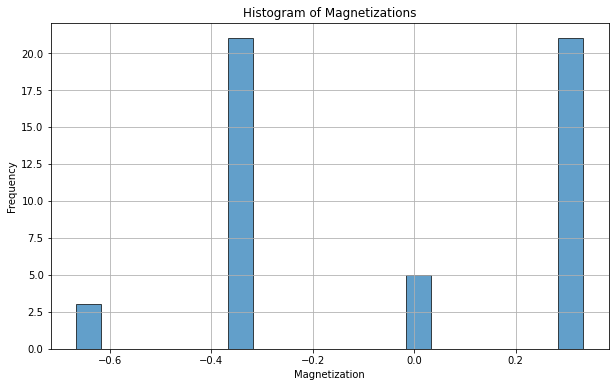
\includegraphics[scale=0.5]{appbHisto.png}
    \caption{A plot showing a histogram of the total magnetization. \newline
    Ideally, we should be seeing total magnetizations only on $\pm$1}
    \label{fig:bHisto}
\end{figure}
\begin{figure}[ht!]
    \centering
    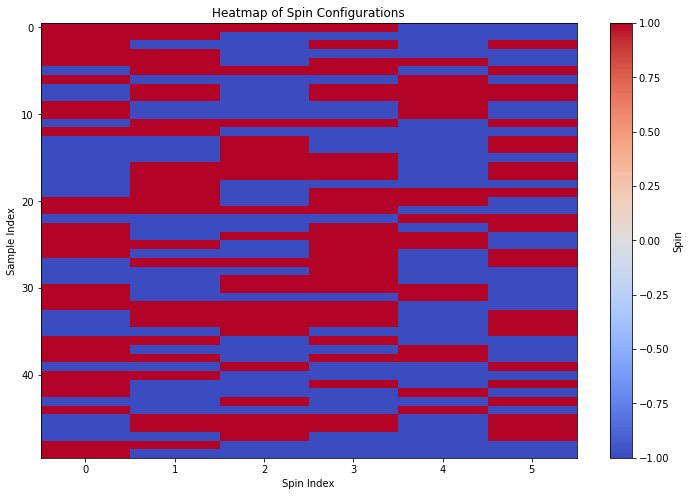
\includegraphics[scale=0.5]{appbConfs.png}
    \caption{A plot showing the configurations of each sample. \newline
    Ideally, we should be seeing uniform (that is one colour) lines across the x-axis}
    \label{fig:bConfs}
\end{figure}
\begin{figure}[ht!]
    \centering
    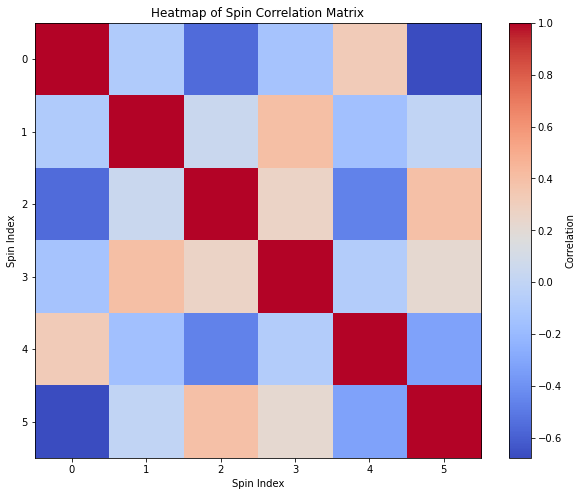
\includegraphics[scale=0.5]{appbCorrs.png}
    \caption{A plot showing the matrix of spin correlations \newline
    Ideally, here we should an entirely red plot, if the spins were correlated with each other}
    \label{fig:bCorrs}
\end{figure}
\newpage
We see here that all figures show results that are not in line with the theory. This is indicative of one of two things. Either something is wrong with out Metropolis-Hastings algorithm for binary inputs, or the Neural Network cannot correctly approximate the wave function such that our sampling algorithm is unable to provide samples from the correct distribution.
\end{document}


